\documentclass[twoside,12pt]{book}

\usepackage{amsmath, amsthm, amssymb, amsfonts}
\usepackage{thmtools}
\usepackage{graphicx}
\usepackage{setspace}
\usepackage{geometry}
\usepackage{float}
\usepackage{hyperref}
\usepackage[backend=bibtex, style=numeric, sorting=none]{biblatex}
\usepackage[utf8]{inputenc}
\usepackage[spanish]{babel}
\usepackage{framed}
\usepackage[dvipsnames]{xcolor}
\usepackage{environ}
\usepackage{tcolorbox}

\tcbuselibrary{theorems,skins,breakable}
\addbibresource{bibliography.bib}

\setstretch{1.0}
\geometry{
    textheight=8.3in,
    textwidth=5.8in,
    top=0.8in,
    inner=1.2in,
    outer=0.8in,
    bottom=0.8in,
    headheight=12pt,
    headsep=25pt,
    footskip=30pt
}

\setlength{\parindent}{0pt}


% Variables
\def\notetitle{Notas: Diseño de Controladores No Lineales}
\def\noteauthor{
    \textbf{Profesor} \\ 
    Dr. Jaime Moreno \\
    \textbf{Autor} \\
    A. León\\
    \\
    Posgrado de Ingeniería, UNAM}
\def\notedate{2025}

% The theorem system and user-defined commands
% Theorem System
% The following boxes are provided:
%   Definition:     \defn 
%   Theorem:        \thm 
%   Lemma:          \lem
%   Corollary:      \cor
%   Proposition:    \prop   
%   \partial:          \clm
%   Fact:           \fact
%   Proof:          \pf
%   Example:        \ex
%   Remark:         \rmk (sentence), \rmkb (block)
% Suffix
%   r:              Allow Theorem/Definition to be referenced, e.g. thmr
%   p:              Add a short proof block for Lemma, Corollary, Proposition or Claim, e.g. lemp
%                   For theorems, use \pf for proof blocks

% Definition
\newtcbtheorem[number within=section]{mydefinition}{Definición}
{
    enhanced,
    breakable,
    frame hidden,
    titlerule=0mm,
    toptitle=1mm,
    bottomtitle=1mm,
    fonttitle=\bfseries\large,
    coltitle=black,
    colbacktitle=green!20!white,
    colback=green!10!white,
}{defn}

\NewDocumentCommand{\defn}{m+m}{
    \begin{mydefinition}{#1}{}
        #2
    \end{mydefinition}
}

\NewDocumentCommand{\defnr}{mm+m}{
    \begin{mydefinition}{#1}{#2}
        #3
    \end{mydefinition}
}

% Theorem
\newtcbtheorem[use counter from=mydefinition]{mytheorem}{Teorema}
{
    enhanced,
    breakable,
    frame hidden,
    titlerule=0mm,
    toptitle=1mm,
    bottomtitle=1mm,
    fonttitle=\bfseries\large,
    coltitle=black,
    colbacktitle=cyan!20!white,
    colback=cyan!10!white,
}{thm}

\NewDocumentCommand{\thm}{m+m}{
    \begin{mytheorem}{#1}{}
        #2
    \end{mytheorem}
}

\NewDocumentCommand{\thmr}{mm+m}{
    \begin{mytheorem}{#1}{#2}
        #3
    \end{mytheorem}
}

% Lemma
\newtcbtheorem[use counter from=mydefinition]{mylemma}{Lema}
{
    enhanced,
    breakable,
    frame hidden,
    titlerule=0mm,
    toptitle=1mm,
    bottomtitle=1mm,
    fonttitle=\bfseries\large,
    coltitle=black,
    colbacktitle=violet!20!white,
    colback=violet!10!white,
}{lem}

\NewDocumentCommand{\lem}{m+m}{
    \begin{mylemma}{#1}{}
        #2
    \end{mylemma}
}

\newenvironment{lempf}{
	{\noindent{\it \textbf{Proof for Lemma}}}
	\tcolorbox[blanker,breakable,left=5mm,parbox=false,
    before upper={\parindent15pt},
    after skip=10pt,
	borderline west={1mm}{0pt}{violet!20!white}]
}{
    \textcolor{violet!20!white}{\hbox{}\nobreak\hfill$\blacksquare$} 
    \endtcolorbox
}

\NewDocumentCommand{\lemp}{m+m+m}{
    \begin{mylemma}{#1}{}
        #2
    \end{mylemma}

    \begin{lempf}
        #3
    \end{lempf}
}

% Corollary
\newtcbtheorem[use counter from=mydefinition]{mycorollary}{Corolario}
{
    enhanced,
    breakable,
    frame hidden,
    titlerule=0mm,
    toptitle=1mm,
    bottomtitle=1mm,
    fonttitle=\bfseries\large,
    coltitle=black,
    colbacktitle=orange!20!white,
    colback=orange!10!white,
}{cor}

\NewDocumentCommand{\cor}{+m}{
    \begin{mycorollary}{}{}
        #1
    \end{mycorollary}
}

\newenvironment{corpf}{
	{\noindent{\it \textbf{Proof for Corollary.}}}
	\tcolorbox[blanker,breakable,left=5mm,parbox=false,
    before upper={\parindent15pt},
    after skip=10pt,
	borderline west={1mm}{0pt}{orange!20!white}]
}{
    \textcolor{orange!20!white}{\hbox{}\nobreak\hfill$\blacksquare$} 
    \endtcolorbox
}

\NewDocumentCommand{\corp}{m+m+m}{
    \begin{mycorollary}{}{}
        #1
    \end{mycorollary}

    \begin{corpf}
        #2
    \end{corpf}
}

% Proposition
\newtcbtheorem[use counter from=mydefinition]{myproposition}{Proposición}
{
    enhanced,
    breakable,
    frame hidden,
    titlerule=0mm,
    toptitle=1mm,
    bottomtitle=1mm,
    fonttitle=\bfseries\large,
    coltitle=black,
    colbacktitle=yellow!30!white,
    colback=yellow!20!white,
}{prop}

\NewDocumentCommand{\prop}{+m}{
    \begin{myproposition}{}{}
        #1
    \end{myproposition}
}

\newenvironment{proppf}{
	{\noindent{\it \textbf{Prueba de la Proposición.}}}
	\tcolorbox[blanker,breakable,left=5mm,parbox=false,
    before upper={\parindent15pt},
    after skip=10pt,
	borderline west={1mm}{0pt}{yellow!50!white}]
}{
    \textcolor{yellow!30!white}{\hbox{}\nobreak\hfill$\blacksquare$} 
    \endtcolorbox
}

\NewDocumentCommand{\propp}{+m+m}{
    \begin{myproposition}{}{}
        #1
    \end{myproposition}

    \begin{proppf}
        #2
    \end{proppf}
}

% Claim
\newtcbtheorem[use counter from=mydefinition]{myclaim}{Afirmación}
{
    enhanced,
    breakable,
    frame hidden,
    titlerule=0mm,
    toptitle=1mm,
    bottomtitle=1mm,
    fonttitle=\bfseries\large,
    coltitle=black,
    colbacktitle=pink!30!white,
    colback=pink!20!white,
}{clm}


\NewDocumentCommand{\clm}{m+m}{
    \begin{myclaim*}{#1}{}
        #2
    \end{myclaim*}
}

\newenvironment{clmpf}{
	{\noindent{\it \textbf{Prueba para afirmación.}}}
	\tcolorbox[blanker,breakable,left=5mm,parbox=false,
    before upper={\parindent15pt},
    after skip=10pt,
	borderline west={1mm}{0pt}{pink!30!white}]
}{
    \textcolor{pink!30!white}{\hbox{}\nobreak\hfill$\blacksquare$} 
    \endtcolorbox
}

\NewDocumentCommand{\clmp}{m+m+m}{
    \begin{myclaim*}{#1}{}
        #2
    \end{myclaim*}

    \begin{clmpf}
        #3
    \end{clmpf}
}

% Fact
\newtcbtheorem[use counter from=mydefinition]{myfact}{Propiedad}
{
    enhanced,
    breakable,
    frame hidden,
    titlerule=0mm,
    toptitle=1mm,
    bottomtitle=1mm,
    fonttitle=\bfseries\large,
    coltitle=black,
    colbacktitle=purple!20!white,
    colback=purple!10!white,
}{fact}

\NewDocumentCommand{\fact}{+m}{
    \begin{myfact}{}{}
        #1
    \end{myfact}
}


% Proof
\NewDocumentCommand{\pf}{+m}{
    \begin{proof}
        [\noindent\textbf{Prueba.}]
        #1
    \end{proof}
}

% Example
\newtcbtheorem[use counter from=mydefinition]{myexample}{Ejemplo}
{
    enhanced,
    breakable,
    frame hidden,
    titlerule=0mm,
    toptitle=1mm,
    bottomtitle=1mm,
    fonttitle=\bfseries\large,
    coltitle=black,
    colbacktitle=black!10!white,
    colback=black!2!white,
}{ex}


\NewDocumentCommand{\ex}{m}{
    % \begin{minipage}{\textwidth}
        \begin{myexample}{}{}
            #1
        \end{myexample}
    % \end{minipage}
}



% Remark
\NewDocumentCommand{\rmk}{+m}{
    {\it \color{blue!90!white}#1}
}

\newenvironment{remark}{
    \par
    \vspace{5pt}
    \begin{minipage}{\textwidth}
        {\par\noindent{\textbf{Observación}}}
        \tcolorbox[blanker,breakable,left=5mm,
        before skip=10pt,after skip=10pt,
        borderline west={1mm}{0pt}{red!40!white}]
}{
        \endtcolorbox
    \end{minipage}
    \vspace{5pt}
}

\NewDocumentCommand{\rmkb}{+m}{
    \begin{remark}
        #1
    \end{remark}
}


\newcommand{\lcm}{\operatorname{lcm}}


\usepackage[acronym]{glossaries}
\makeglossaries
\newacronym{gr}{GR}{Grado Relativo}
\newacronym{siso}{SISO}{Single Input Single Output}
\newacronym{si}{SI}{Single Input}
\newacronym{dc}{DC}{Dinámica Cero}
\newacronym{edp}{EDP}{Ecuación Diferencial Parcial}
\newacronym{fn}{FN}{Forma Normal (de Byrnes-Isidori)}
\newacronym{fc}{FC}{Forma de Controlador}
\newacronym{flc}{FLC}{Función de Lyapunov de Control}
\newacronym{fl}{FL}{Función de Lyapunov}
\newacronym{rna}{RNA}{Radialmente no Acotada}
\newacronym{pcp}{PCP}{Propiedad de Control Pequeño}
\newacronym{lit}{LIT}{Lineal e Invariante en el Tiempo}
\newacronym{pe}{PE}{Punto de Equilibrio}
\newacronym{gae}{GAE}{Global y Asintóticamente Estable}
\newacronym{gee}{GEE}{Global y Exponencialmente Estable}


% ------------------------------------------------------------------------------

\begin{document}
\title{\textbf{
		\LARGE{\notetitle} \vspace*{10\baselineskip}}
}
\author{\noteauthor}
\date{\notedate}

\maketitle
\newpage

\tableofcontents
\newpage

\printglossary[type=\acronymtype, title=Lista de Acrónimos]
\newpage

% ------------------------------------------------------------------------------

%%%%%%%%%%%%%%%%%%%%%%%%%%%%%%%%%%%%%%%%%%%%%%%%%%%%%%%%%%%%%%%%%%%%%%%%%%%%%%%%%%%%%%%%%%%%%%%%%%%%%%%
% Capítulo 1: Grado Relativo, Forma Normal y Dinámica Cero
%%%%%%%%%%%%%%%%%%%%%%%%%%%%%%%%%%%%%%%%%%%%%%%%%%%%%%%%%%%%%%%%%%%%%%%%%%%%%%%%%%%%%%%%%%%%%%%%%%%%%%%

\chapter{Grado relativo, Forma Normal y Dinámica Cero}

\section{Grado Relativo}

El \gls{gr} de un sistema tiene que ver con el hecho de que si nosotros derivamos la salida iterativamente, eventualmente en alguna de esas derivadas vamos a encontrar la acción de la entrada. La derivada más pequeña para la cual eso ocurre es el \gls{gr}.\\

De manera más formal, considere el siguiente sistema no lineal \gls{siso} afín en la entrada:

\begin{equation}
	\begin{aligned}
		\dot{x} & = f(x) + g(x)u \\
		y       & = h(x) \, ,
	\end{aligned}
	\label{eq:siso_afin}
\end{equation}

donde
\begin{itemize}
	\item $f, g$ y $h$ son funciones suaves en un dominio $D \subseteq \mathbb{R}^n$.
	\item $f: D \rightarrow \mathbb{R}^n$ y $g: D \rightarrow \mathbb{R}^{n}$ son campos vectoriales en $D$.
\end{itemize}

Tomamos la derivada de la salida, haciendo uso de la regla de la cadena:

\begin{equation*}
	\begin{aligned}
		\dot{y} & = \dfrac{\partial h(x)}{\partial x} \dot{x}                                        \\
		        & = \dfrac{\partial h(x)}{\partial x} f(x) + \dfrac{\partial h(x)}{\partial x} g(x)u \\
		        & \overset{\Delta}{=} L_fh(x) + L_gh(x)u \, ,
	\end{aligned}
\end{equation*}

donde
\begin{equation*}
	L_fh(x) = \dfrac{\partial h(x)}{\partial x} f(x)
\end{equation*}
es la \textit{Derivada de Lie} de $h$ con respecto a $f$ o a lo largo de $f$.\\

Entonces, para el sistema \ref{eq:siso_afin}, si tomamos la primera derivada de la salida:
\begin{equation*}
	\dot{y} = L_fh(x) + L_gh(x)u \, ,
\end{equation*}
si
\begin{equation*}
	L_gh(x) = 0 \quad \Rightarrow \quad \dot{y} = L_fh(x) \, ,
\end{equation*}
y notamos que la primera derivada de la salida no depende de la entrada $u$. Tomando una derivada más:
\begin{equation*}
	y^{(2)} = \ddot{y} = L_f^2h(x) + L_g L_fh(x)u \, ,
\end{equation*}
si
\begin{equation*}
	L_g L_fh(x) = 0 \quad \Rightarrow \quad y^{(2)}  = L_f^2h(x) \, ,
\end{equation*}
nuevamente la segunda derivada de la salida no depende de la entrada $u$. Derivamos una vez más:
\begin{equation*}
	y^{(3)} = \dddot{y} = L_f^3h(x) + L_g L_f^2h(x)u \, ,
\end{equation*}
si
\begin{equation*}
	L_g L_f^2h(x) = 0 \quad \Rightarrow \quad y^{(3)} = L_f^3h(x) \, .
\end{equation*}
Generalizando, si
\begin{equation*}
	\begin{aligned}
		L_g L_f^{i-1} h(x)    & = 0, \quad i = 1, 2, \ldots, \rho-1; \\
		L_g L_f^{\rho-1} h(x) & \neq 0 \, ,
	\end{aligned}
\end{equation*}
entonces
\begin{equation*}
	\begin{aligned}
		y^{(i)} = L_f^i h(x), \quad i = 1, 2, \ldots, \rho-1; \\
		y^{(\rho)} = L_f^\rho h(x) + L_g L_f^{\rho-1} h(x)u \, .
	\end{aligned}
\end{equation*}

\defn{Grado Relativo}{
	El sistema \gls{siso} afín en la entrada \ref{eq:siso_afin} tiene \gls{gr} $\rho$, con $1 \leq \rho \leq n$, en $D_0 \subset D \subseteq \mathbb{R}^n$ si $ \forall x \in D_0$ se cumple que

	\begin{equation}
		\begin{aligned}
			L_g L_f^{i-1} h(x)    & = 0, \quad i = 1, 2, \ldots, \rho-1; \\
			L_g L_f^{\rho-1} h(x) & \neq 0 \, .
		\end{aligned}
		\label{eq:gr}
	\end{equation}
}

\ex{
	\[
		\begin{aligned}
			 & \dot{x}_1 = x_2                                                   \\
			 & \dot{x}_2 = -x_1 + \epsilon(1 - x_1^2)x_2 + u, \quad \epsilon > 0 \\
			 & y = x_1
		\end{aligned}
	\] \\
	\[
		\dot{y} = \dot{x}_1 = x_2
	\] \\
	\[
		\ddot{y} = \dot{x}_2 = -x_1 + \epsilon(1 - x_1^2)x_2 + u
	\] \\
	El \gls{gr} $= 2$ sobre $D = \mathbb{R}^2$.
}
\newpage

\ex{
	\[
		\begin{aligned}
			 & \dot{x}_1 = x_2                                                   \\
			 & \dot{x}_2 = -x_1 + \epsilon(1 - x_1^2)x_2 + u, \quad \epsilon > 0 \\
			 & y = x_2
		\end{aligned}
	\] \\
	\[
		\dot{y} = \dot{x}_2 = -x_1 + \epsilon(1 - x_1^2)x_2 + u
	\] \\
	El \gls{gr} $= 1$ sobre $D = \mathbb{R}^2$.
}

\ex{
	\[
		\begin{aligned}
			 & \dot{x}_1 = x_2                                                   \\
			 & \dot{x}_2 = -x_1 + \epsilon(1 - x_1^2)x_2 + u, \quad \epsilon > 0 \\
			 & y = x_1 + x_2^2
		\end{aligned}
	\] \\
	\[ \begin{aligned}
			\dot{y} & = \dot{x}_1 + 2x_2\dot{x}_2                          \\
			        & = x_2 -2x_1x_2 + 2 \epsilon (1 - x_1^2)x_2^2 + 2x_2u
		\end{aligned} \] \\
	El \gls{gr} $= 1$ sobre $D_0 = \{  x\in\ \mathbb{R}^2 \, | \, x_2 \neq 0 \}$.
}

\ex{
	\textbf{Motor de corriente directa controlado por campo}
	\[
		\begin{aligned}
			 & \dot{x}_1 = -ax_1 + u           \\
			 & \dot{x}_2 = -bx_2 + k - cx_1x_3 \\
			 & \dot{x}_3 = \theta x_1 x_2      \\
			 & y = x_3
		\end{aligned}
	\] \\
	con $a, b, c, k, \theta > 0$.\\
	\[
		\begin{aligned}
			\dot{y} & = \dot{x}_3 = \theta x_1 x_2
		\end{aligned}
	\] \\
	\[
		\begin{aligned}
			\ddot{y} & = \theta \dot{x}_1 x_2 + \theta x_1 \dot{x}_2                                       \\
			         & = \left[ -a\theta x_1 x_2 + \theta x_1 (-bx_2 + k - cx_1x_3) \right] + \theta x_2 u
		\end{aligned}
	\] \\
	El \gls{gr} $= 2$ sobre $D_0 = \{ x \in \mathbb{R}^2 \, | \, x_2 \neq 0 \}$.
}

\section{Forma Normal}

Si un sistema tiene \gls{gr} bien definido, siempre se puede llevar a una forma especial, esta es la \gls{fn}\\

Para el sistema \gls{siso}
\begin{equation}
	\begin{aligned}
		\dot{x} & = f(x) + g(x)u \\
		y       & = h(x) \, ,
	\end{aligned}
	\label{eq:siso}
\end{equation}
con \gls{gr} $\rho$, $1 \leq \rho \leq n$, en $D_0 \subset D \subseteq \mathbb{R}^n$ \textit{bien definido}, esto es,
\begin{equation}
	\begin{aligned}
		L_g L_f^{i-1} h(x)    & = 0, \quad i = 1, 2, \ldots, \rho-1; \quad \forall x \in D_0 \\
		L_g L_f^{\rho-1} h(x) & \neq 0 ; \quad \forall x \in D_0 \, ,
	\end{aligned}
	\label{eq:gr2}
\end{equation}
se puede encontrar un difeomorfismo (función invertible, suave y con inversa suave) construido de la siguiente manera:
\begin{equation}
	z = T(x) = \begin{bmatrix}
		\phi_1(x)         \\
		\vdots            \\
		\phi_{n-\rho}(x)  \\
		- - -             \\
		h(x)              \\
		\vdots            \\
		L_f^{\rho-1} h(x) \\
	\end{bmatrix} \overset{\Delta}{=} \begin{bmatrix}
		\phi(x) \\
		- - -   \\
		\psi(x)
	\end{bmatrix} \overset{\Delta}{=} \begin{bmatrix}
		\eta  \\
		- - - \\
		\xi
	\end{bmatrix} \, .
	\label{eq:difeomorfismo}
\end{equation}

Observamos que $z$ es un vector compuesto por $n$ funciones escalares. De estas, las últimas $\rho$ están determinadas de manera única por la salida $y$ y sus derivadas de Lie a lo largo de $f$ hasta el orden $\rho-1$. En cambio, las $n-\rho$ funciones restantes, denotadas como $ \phi_1(x), \ldots , \phi_{n-\rho}(x) $, se eligen de manera que $T(x)$ sea un difeomorfismo en un dominio $\bar{D_0} \subset D_0 \subset D$.  \\

Para garantizar que $T(x)$ sea un difeomorfismo, las funciones $\phi$ deben ser \textit{linealmente independientes}, es decir, sus gradientes deben ser linealmente independientes. Esto se debe a que una función es localmente invertible si su \textit{jacobiano} es una matriz regular, lo que sigue del \textit{teorema de la función inversa}.\\

Finalmente, notamos que el vector $z$ lo descomponemos en una componente $\eta$ y otra $\xi$. Entonces, la dinámica del sistema en las nuevas coordenadas es:
\begin{equation}
	\begin{aligned}
		\dot{\eta}     & = \dfrac{\partial \phi(x)}{\partial x} \left[ f(x) + g(x)u \right] = f_0(\eta, \xi) + g_0(\eta, \xi)u \\
		\dot{\xi}_i    & = \dfrac{\partial L_f^{i-1} h(x)}{\partial x} \left[ f(x) + g(x)u \right]                             \\
		               & = L_f^i h(x) + L_g L_f^{i-1} h(x)u = \xi_{i+1}, \quad  1 \leq i \leq \rho-1                           \\
		\dot{\xi}_\rho & = L_f^\rho h(x) + L_g L_f^{\rho-1} h(x)u                                                              \\
		y              & = \xi_1 \, .
	\end{aligned}
	\label{eq:siso_normal}
\end{equation}

Elíjase $\phi(x)$ tal que $T(x)$ sea un difeomorfismo y
\begin{equation}
	\dfrac{\partial \phi_i(x)}{\partial x} g(x) = 0, \quad 1 \leq i \leq n-\rho; \quad \forall x \in \bar{D}_0 \, ,
\end{equation}
es decir, buscamos que el gradiente de $\phi(x)$ sea ortogonal a $g(x)$, esto se puede lograr seleccionando adecuadamente las funciones $\phi_i(x)$.\\

\rmk{
	¿Cuántos vectores linealmente independientes podemos elegir ortogonales a $g(x)$? \\

	Se pueden elegir $n - 1$, pues $g(x)$ es un vector de dimensión $n$, y su espacio ortogonal es un plano de dimensión $n-1$. \\

	¿Y aquí cuántos tenemos que elegir? \\

	Debemos elegir $n - \rho$.\\
}

\rmkb{Esto siempre es posible, al menos localmente. Es decir, es posible elegir las $\phi_i$ funciones linealmente independientes, y adicionalmente, escogerlas ortogonales a $g(x)$, al menos en un dominio $\bar{D}_0$.}

\thm{}{
Suponga que el sistema \gls{siso}
\begin{equation*}
	\begin{aligned}
		\dot{x} & = f(x) + g(x)u \\
		y       & = h(x) \, ,
	\end{aligned}
\end{equation*}
tiene \gls{gr} $\rho$, $1 \leq \rho \leq n$, en $D_0 \subset D \subseteq \mathbb{R}^n$.
\begin{itemize}
	\item Si $\rho = n$, entonces, $\forall \bar{x} \in D_0$, existe una vecindad $\mathcal{N}_{\bar{x}}$ de $\bar{x}$ tal que el mapa $\psi(x)$, restringido a $\mathcal{N}_{\bar{x}}$, es un \textbf{difeomorfismo} en $\mathcal{N}_{\bar{x}}$.
	\item Si $\rho < n$, entonces, $\forall \bar{x} \in D_0$, existen
	      \begin{itemize}
		      \item una \textbf{vecindad} $\mathcal{N}_{\bar{x}}$ de $\bar{x}$, y
		      \item funciones suaves $\phi_1(x), \ldots, \phi_{n-\rho}(x)$,
	      \end{itemize}
\end{itemize}
tales que
\begin{equation*}
	\dfrac{\partial \phi_i(x)}{\partial x} g(x) = 0, \quad 1 \leq i \leq n-\rho; \quad \forall x \in \mathcal{N}_{\bar{x}} \, ,
\end{equation*}
y el mapa
\begin{equation*}
	z = T(x) = \begin{bmatrix}
		\phi(x) \\
		- - -   \\
		\psi(x)
	\end{bmatrix} \; ,
\end{equation*}
restringido a $\mathcal{N}_{\bar{x}}$, es un \textbf{difeomorfismo} en $\mathcal{N}_{\bar{x}}$.\\

En tal caso, el sistema en las nuevas coordenadas queda en la \gls{fn}:
\begin{equation}
	\text{Forma Normal:}
	\begin{cases}
		\dot{\eta} = f_0(\eta, \xi)                            \\
		\dot{\xi_i} = \xi_{i+1}, \quad 1 \leq i \leq \rho-1    \\
		\dot{\xi_\rho} = L_f^\rho h(x) + L_g L_f^{\rho-1}h(x)u \\
		y = \xi_1
	\end{cases} \; ,
	\label{eq:forma_normal}
\end{equation}
o en forma más compacta
\begin{equation}
	\text{Forma Normal:}
	\begin{cases}
		\dot{\eta} = f_0(\eta, \xi)                        \\
		\dot{\xi} = A_c \xi + B_c \gamma(x)[u - \alpha(x)] \\
		y = C_c \xi
	\end{cases} \; ,
	\label{eq:forma_normal_compacta}
\end{equation}
donde,
\begin{equation*}
	A_c = \begin{bmatrix}
		0      & 1      & 0      & \ldots & 0      \\
		0      & 0      & 1      & \ldots & 0      \\
		\vdots & \vdots & \vdots & \ddots & \vdots \\
		0      & 0      & 0      & \ldots & 1      \\
		0      & 0      & 0      & \ldots & 0
	\end{bmatrix} \; , \quad B_c = \begin{bmatrix}
		0      \\
		0      \\
		\vdots \\
		0      \\
		1
	\end{bmatrix} \; , \quad C_c = \begin{bmatrix}
		1 & 0 & 0 & \ldots & 0
	\end{bmatrix} \; ,
\end{equation*}
\begin{equation*}
	\gamma(x) = L_g L_f^{\rho-1} h(x) \; , \quad \alpha(x) = -\dfrac{L_f^\rho h(x)}{L_g L_f^{\rho-1} h(x)} \; .
\end{equation*}
}

\section{Dinámica Cero}

El concepto de \gls{dc} es independiente del sistema de coordenadas, pero su estudio se simplifica considerablemente en la \gls{fn}.\\

Cuando hablamos de la \gls{dc} de un sistema, nos referimos a la evolución del sistema cuando la salida se mantiene en cero. Es natural pensar que esto se logra anulando la entrada, pero esto no siempre es cierto ni es la única forma de conseguirlo; de hecho, existen infinitas maneras de forzar la salida a cero. Así, la \gls{dc} describe todas las posibles trayectorias del sistema, junto con sus respectivas entradas, que garantizan que la salida permanezca nula de manera unívoca.\\

Considere el sistema \gls{siso} en la \gls{fn}:
\begin{equation*}
	\begin{cases}
		\dot{\eta} = f_0(\eta, \xi)                        \\
		\dot{\xi} = A_c \xi + B_c \gamma(x)[u - \alpha(x)] \\
		y = C_c \xi
	\end{cases} \; .
\end{equation*}
Si la salida es \textbf{cero} durante un intervalo de tiempo $t \in (0, T)$, entonces durante este intervalo
\begin{equation*}
	\begin{aligned}
		y(t) \equiv 0 \quad & \Rightarrow \quad y^{(i)}(t) = 0, \quad i = 1, 2, \; \ldots \quad \Rightarrow \quad \xi(t) \equiv 0 \\
		                    & \Rightarrow \quad u(t) \equiv \alpha(x(t)) \quad \Rightarrow \quad \dot{\eta} = f_0(\eta, 0) \, .
	\end{aligned}
\end{equation*}
Note que en la \gls{fn}, las derivadas de la salida son variables de estado (las variables $\xi$), por lo que la solo nos queda determinar la dinámica de $\dot{\eta}$.\\

\defn{Dinámica Cero}{
	La ecuación
	\begin{equation}
		\dot{\eta} = f_0(\eta, 0)
		\label{eq:dc}
	\end{equation}
	se denomina la \textbf{Dinámica Cero} del sistema.\\

	Adicionalmente, se dice que el sistema es de \textbf{Fase Mínima} si la dinámica cero tiene un punto de equilibrio asintóticamente estable en el dominio de interés (en el origen si $T(0)=0$).
}

\rmkb{
	La \gls{dc} corresponde a todas las parejas de condiciones iniciales y entradas al sistema que hacen que la salida sea cero. En la \gls{fn} esto es especialmente simple:
	\begin{equation*}
		\begin{aligned}
			\text{Si } \quad (\eta_0, \xi_0) & = (\eta_0, 0) \; \text{ y } \; u(t) \equiv \alpha(x(t)), \quad \text{donde} \\
			                                 & x(t) = T^{-1} \left( \begin{bmatrix}
					                                                        \eta_0 \\
					                                                        0
				                                                        \end{bmatrix} \right) y                                \\
			                                 & \dot{\eta}(t) = f_0(\eta(t), 0), \; \eta(0) = \eta_0                        \\
			\text{Entonces}                  & \quad \Rightarrow y(t) \equiv 0 \, .
		\end{aligned}
	\end{equation*}
}
\rmkb{
	En las coordenadas originales la \gls{dc} puede caracterizarse de la siguiente manera:
	\begin{equation*}
		Z^* = \left\{ x \in \bar{D}_0 \, | \, h(x) = L_f h(x) = \ldots = L_f^{\rho-1} h(x) = 0 \right\} \, ,
	\end{equation*}
	Entonces
	\begin{equation*}
		\begin{aligned}
			y(t)  \equiv 0 \quad & \Rightarrow \quad x(t) \in Z^*                                                  \\
			                     & \Rightarrow \quad u(t) = u^*(x) \overset{\Delta}{=} \alpha(x) \, |_{x\in Z^*} \
		\end{aligned}
	\end{equation*}
	La dinámica restringida del sistema se describe como
	\begin{equation*}
		\dot{x} = f^*(x) \overset{\Delta}{=} \left[ f(x) + g(x)\alpha(x) \right]_{x\in Z^*} \, .
	\end{equation*}
}
\newpage
\ex{
	\[
		\begin{aligned}
			 & \dot{x}_1 = x_2                                                   \\
			 & \dot{x}_2 = -x_1 + \epsilon(1 - x_1^2)x_2 + u, \quad \epsilon > 0 \\
			 & y = x_2
		\end{aligned}
	\] \\
	\[
		\begin{aligned}
			\dot{y}       & = \dot{x}_2 = -x_1 + \epsilon(1 - x_1^2)x_2 + u \; \Rightarrow \; \rho = 1                                 \\
			y(t) \equiv 0 & \quad \Rightarrow \quad x_2(t) \equiv 0 \; \Rightarrow \; \dot{x}_1(t) = 0 \; \Rightarrow \; u(t) = 0 \, .
		\end{aligned}
	\]\\
	El sistema es de Fase No Mínima.
}

\ex{
\[
	\begin{aligned}
		 & \dot{x}_1 = -x_1 + \dfrac{2 + x_3^2}{1 + x_3^2}u \\
		 & \dot{x}_2 = x_3                                  \\
		 & \dot{x}_3 = x_1 x_3 + u                          \\
		 & y = x_2
	\end{aligned}
\] \\
\[
	\begin{aligned}
		\dot{y}  & = \dot{x}_2 = x_3                                    \\
		\ddot{y} & = \dot{x}_3 = x_1 x_3 + u \; \Rightarrow \; \rho = 2 \\
	\end{aligned}
\]\\
\[
	\gamma(x) = L_g L_f h(x) = 1 \; , \quad \alpha(x) = -\dfrac{L_f^{\rho} h(x)}{L_g L_f^{\rho-1} h(x)} = -x_1x_3 \;
\]\\
\[
	\begin{aligned}
		Z^*       & = \left\{ x_2 = x_3 = 0 \right\} \\
		u         & = u^*(x) = 0                     \\
		\dot{x}_1 & = -x_1 \; .
	\end{aligned}
\]\\
El sistema es de Fase Mínima.\\
\\
\rmk{¿Cuál es la transformación para llevar al sistema a la \gls{fn}?}\\
\\
Hay que hallar $\phi(x)$ tal que
\[
	\begin{aligned}
		\phi(0) & = 0, \; \dfrac{\partial \phi(x)}{\partial x} g(x) = 0                                                                                                                              \\
		        & = \left[ \dfrac{\partial \phi(x)}{\partial x_1} \, , \, \dfrac{\partial \phi(x)}{\partial x_2} \, , \, \dfrac{\partial \phi(x)}{\partial x_3} \right] \begin{bmatrix}
			                                                                                                                                                                \dfrac{2 + x_3^2}{1 + x_3^2} \\
			                                                                                                                                                                0                            \\
			                                                                                                                                                                1
		                                                                                                                                                                \end{bmatrix} = 0
	\end{aligned}
\]
y
\[
	T(x) = \begin{bmatrix}
		\phi(x) \\
		h(x)    \\
		L_f h(x)
	\end{bmatrix}
\]
sea un difeomorfismo.\\
\[
	\dfrac{\partial\phi(x)}{\partial x}g(x) = \dfrac{\partial\phi(x)}{\partial x_1} \dfrac{2+x_3^2}{1+x_3^2} + \dfrac{\partial\phi(x)}{\partial x_3} = 0
\]
La función
\[
	\phi(x) = -x_1 + x_3 + \tan^{-1}(x_3)
\]
satisface la \gls{edp} y $\phi(0)=0$.\\
\[
	T(x) = \begin{bmatrix}
		\eta  \\
		\xi_1 \\
		\xi_2
	\end{bmatrix} = \begin{bmatrix}
		-x_1 + x_3 + \tan^{-1}(x_3) \\
		x_2                         \\
		x_1x_3
	\end{bmatrix}
\]
es un difeomorfismo global. La \gls{fn} es entonces
\[
	\begin{cases}
		\dot{\eta} = (-\eta + \xi_2 + \tan^{-1}(\xi_2))\left( 1 + \dfrac{2 + \xi_2^2}{1 + \xi_2^2}\xi_2^2 \right) \\
		\dot{\xi}_1 = \xi_2                                                                                       \\
		\dot{\xi}_2 = (-\eta + \xi_2 + \tan^{-1}(\xi_2))\xi_2 + u                                                 \\
		y = \xi_1
	\end{cases}
\]
}

%%%%%%%%%%%%%%%%%%%%%%%%%%%%%%%%%%%%%%%%%%%%%%%%%%%%%%%%%%%%%%%%%%%%%%%%%%%%%%%%%%%%%%%%%%%%%%%%%%%%%%%
% Capítulo 2: Forma de Controlador
%%%%%%%%%%%%%%%%%%%%%%%%%%%%%%%%%%%%%%%%%%%%%%%%%%%%%%%%%%%%%%%%%%%%%%%%%%%%%%%%%%%%%%%%%%%%%%%%%%%%%%%

\chapter{Forma de Controlador}
\section{Forma de Controlador}
\defn{Forma de Controlador}{
	Se dice que un sistema no lineal (con múltiples entradas) está en la \gls{fc} si se puede escribir como
	\begin{equation}
		\dot{x} = Ax + B\gamma(x)[u - \alpha(x)] \, ,
		\label{eq:forma_controlador}
	\end{equation}
	donde
	\begin{itemize}
		\item $(A, B)$ es controlable, $A \in \mathbb{R}^{n \times n}$, $B \in \mathbb{R}^{n \times p}$.
		\item $\gamma(x)$, con $\gamma: D \subset \mathbb{R}^n \rightarrow \mathbb{R}^{p\times p}$, es una matriz no singular para cada $x \in D$.
	\end{itemize}
}

\rmkb{Note que todas las no linealidades están en el mismo canal que la entrada. La dinámica no lineal del sistema se puede manipular libremente.}

\fact{
	Un sistema que está en la \gls{fc} se puede linealizar exactamente mediante retroalimentación de los estados:\\

	Si se elige
	\begin{equation*}
		u = \alpha(x) + \gamma^{-1}(x) v \, ,
	\end{equation*}
	donde
	\begin{itemize}
		\item $\gamma^{-1}(x)$ es la inversa de $\gamma(x)$, y
		\item $v$ es la entrada de control,
	\end{itemize}
	entonces la dinámica del sistema en lazo cerrado es

	\begin{equation*}
		\dot{x} = Ax + Bv \, ,
	\end{equation*}
	que es lineal en los estados y en la entrada $v$.
}
\defn{Linealizable por Retroalimentación}{
	Se dice que un sistema no lineal
	\begin{equation*}
		\dot{x} = f(x) + G(x)u \, ,
	\end{equation*}
	donde $f: D \rightarrow \mathbb{R}^n$ y $G: D \rightarrow \mathbb{R}^{n \times p}$ son suficientemente suaves en un dominio $D \subseteq \mathbb{R}^n$, es \textbf{Linealizable por Retroalimentación} (o Linealizable Entrada-Estados) si existe un difeomorfismo $T : D \rightarrow \mathbb{R}^n$ tal que
	\begin{itemize}
		\item $D_z = T(D)$ contiene el origen, y
		\item el cambio de variable $z=T(x)$ lleva al sistema a la \gls{fc}.
	\end{itemize}
}

\propp{
	El sistema de dimensión $n$ y con una entrada ($p=1$)
	\begin{equation*}
		\dot{x} = f(x) + g(x)u
	\end{equation*}
	puede ser transformado a la \gls{fc} mediante una transformación de estados $z=T(x)$ si y solo si existe una función (de salida) $h(x)$ tal que el sistema \gls{siso}
	\begin{equation*}
		\begin{aligned}
			\dot{x} & = f(x) + g(x)u \\
			y       & = h(x)
		\end{aligned}
	\end{equation*}
	tenga grado relativo completo, i.e., $\rho = n$.
}{
	$\Leftarrow$: Si el sistema tiene grado relativo $\rho = n$, entonces se puede llevar a la \gls{fn}, que en este caso se reduce a la \gls{fc}, pues no hay porción $\eta$
	\begin{equation*}
		\begin{aligned}
			\dot{\xi} & = A_c \xi + B_c \gamma(x)[u - \alpha(\xi)] \\
			y         & = C_c \xi
		\end{aligned}
	\end{equation*}
	\\
	$\Rightarrow$: Si el sistema se puede transformar a la \gls{fc} mediante una transformación $z=S(x)$, entonces
	\begin{equation*}
		\dot{z} = Az + B \bar{\gamma}(z)[u - \bar{\alpha}(z)].
	\end{equation*}
	Como $(A,B)$ es controlable, entonces existe una matriz regular $M \in \mathbb{R}^{n \times n}$ tal que
	\begin{equation*}
		\begin{aligned}
			MAM^{-1} & = A_c + B_c \lambda^T \\
			MB       & = B_c
		\end{aligned} \, ,
	\end{equation*}
	donde
	\begin{equation*}
		A_c = \begin{bmatrix}
			0      & 1      & 0      & \ldots & 0      \\
			0      & 0      & 1      & \ldots & 0      \\
			\vdots & \vdots & \vdots & \ddots & \vdots \\
			0      & 0      & 0      & \ldots & 1      \\
			0      & 0      & 0      & \ldots & 0
		\end{bmatrix} \; , \quad B_c = \begin{bmatrix}
			0      \\
			0      \\
			\vdots \\
			0      \\
			1
		\end{bmatrix} \; .
	\end{equation*}
	Por lo tanto, la transformación
	\begin{equation*}
		\xi = Mz = MS(x) \overset{\Delta}{=} T(x)
	\end{equation*}
	transforma al sistema a la forma
	\begin{equation*}
		\dot{\xi} = A_c \xi + B_c \gamma(x)[u - \alpha(x)] \, ,
	\end{equation*}
	donde
	\begin{equation*}
		\gamma(x) = \bar{\gamma}(x) \, , \quad \alpha(x) = \bar{\alpha}(x) - \lambda^T M \dfrac{S(x)}{\gamma(x)} \, .
	\end{equation*}
	Eligiendo
	\begin{equation*}
		y = C_c \xi = \xi_1 = T_1(x) = h(x)
	\end{equation*}
	el sistema tiene \gls{gr} $\rho = n$.
}

\section{Condiciones de existencia de $h(x)$}
Ahora nos concentraremos en el problema de hallar una salida con \gls{gr} $\rho = n$.\\

Trataremos de encontrar una caracterización a partir de la cual, con solo mirar la $f(x)$ y $g(x)$, y haciendo ciertas operaciones, decidir si existe un difeomorfismo que lleve a la \gls{fc}.\\

¿Cómo decidir si existe una función suave $h(x)$ tal que
\begin{equation}
	\begin{aligned}
		L_g L_f^{i-1} h(x) & = 0, \quad i = 1, 2, \ldots, n-1; \quad \forall x \in D_0 \\
		L_g L_f^{n-1} h(x) & \neq 0
	\end{aligned}
	\label{eq:edp_h}
\end{equation}
y
\begin{equation*}
	T(x) = \begin{bmatrix}
		h(x)     \\
		L_f h(x) \\
		\vdots   \\
		L_f^{n-1} h(x)
	\end{bmatrix}
\end{equation*}
sea un difeomorfismo?\\

Note que esto termina siendo un problema de resolver una \gls{edp}, que en general es muy complicado. Podemos conformarnos inicialmente en saber si \textbf{existe} una función $h(x)$ que cumpla con las condiciones.\\

Para este fin, es necesario introducir herramientas adicionales.\\

\subsection{El paréntesis de Lie}
\defn{Paréntesis de Lie}{
	El \textbf{paréntesis de Lie} de dos campos vectoriales $f$ y $g$ es un tercer campo vectorial definido como
	\begin{equation}
		[f, g] = \dfrac{\partial g(x)}{\partial x} f(x) - \dfrac{\partial f(x)}{\partial x} g(x) \, .
		\label{eq:lie_bracket}
	\end{equation}
}
Para simplificar la notación, se puede escribir
\begin{equation}
	\begin{aligned}
		 & ad_f^0 g(x) = g(x)                      \\
		 & ad_f g(x) = [f, g](x)                   \\
		 & ad_f^k g(x) = [f, ad_f^{k-1} g](x) \, .
	\end{aligned}
	\label{eq:lie_bracket_simplified}
\end{equation}
Además, algunas propiedades del paréntesis de Lie son
\begin{itemize}
	\item $ [f, g] = -[g, f] $
	\item  Para campos vectoriales constantes $ f, g, \; [f, g] = 0$
\end{itemize}

\subsection{Distribuciones}
Partiendo de la idea de un campo escalar, el cual es una función que asigna un número a cada punto del espacio, podemos decir, de manera informal, que una distribución es un campo en el que a cada punto del espacio se asigna un subespacio. Usualmente, lo hacemos asignando a cada punto un conjunto de vectores que generan el subespacio.

\defn{Distribución}{
	Para los campos vectoriales $f_1, f_2, \ldots, f_k$ en $D \subset \mathbb{R}^n$, sea
	\begin{equation*}
		\Delta(x) = \text{span}\{f_1(x), f_2(x), \ldots, f_k(x)\}
	\end{equation*}
	el espacio vectorial generado por los vectores $f_1(x), f_2(x), \ldots, f_k(x)$.
	La colección de espacios vectoriales $\Delta(x)$ para todo $x \in D$ se llama una \textbf{Distribución} y nos referimos a ella como
	\begin{equation*}
		\Delta = \text{span}\{f_1, f_2, \ldots, f_k\} \, .
	\end{equation*}
	\begin{itemize}
		\item Si la $\text{dim}(\Delta(x)) = k$ para todo $x \in D$, se dice que $\Delta$ es una \textbf{Distribución no singular} (o regular) en $D$, generada por los campos vectoriales $f_1, f_2, \ldots, f_k$.
		\item La distribución es \textbf{Involutiva} si
		      \begin{equation*}
			      g_1 \in \Delta \; \text{y} \; g_2 \in \Delta \quad \Rightarrow \quad [g_1, g_2] \in \Delta
		      \end{equation*}
	\end{itemize}
}

\lem{}{
	Si $\Delta$ es una distribución regular en $D$, generada por $f_1, f_2, \ldots, f_k$, entonces es involutiva si y solo si
	\begin{equation}
		[f_i, f_j] \in \Delta, \quad \forall 1 \leq i, j \leq k \, .
		\label{eq:involutiva}
	\end{equation}
}

\thm{Teorema de Linealización}{
	\label{thm:linealizacion}
	El sistema de dimensión $n$ con una sola entrada \gls{si}
	\begin{equation}
		\dot{x} = f(x) + g(x)u
		\label{eq:si}
	\end{equation}
	es transformable a la \gls{fc} si y solo si existe un dominio $D_0$ tal que
	\begin{enumerate}
		\item $\text{rank} [g(x), ad_f g(x), \ldots, ad_f^{n-1} g(x)] = n, \quad \forall x \in D_0$, y
		\item $\text{span} \{g(x), ad_f g(x), \ldots, ad_f^{n-2} g(x)\}$ es involutiva en $D_0$.
	\end{enumerate}
}

\ex{
\[
	\dot{x} = \begin{bmatrix}
		a \sin x_2 \\
		-x_1 ^2
	\end{bmatrix} + \begin{bmatrix}
		0 \\
		1
	\end{bmatrix} u
\]
\[
	\text{ad}_f g(x) = [f,g] = - \dfrac{\partial f}{\partial x}g = \begin{bmatrix}
		-a \cos x_1 \\
		0
	\end{bmatrix}
\]
Note que el procedimiento para encontrar difeomorfismo de estados que transforme al istema a su \gls{fc} consiste en los siguientes pasos:
\begin{enumerate}
	\item A partir de $f$ y $g$, construir los campos vectoriales
	      \[
		      \text{ad}_f g(x), \; \ldots \; , \text{ad}_f^{n-2} g(x), \; \text{ad}_f^{n-1} g(x)
	      \]
	      y verificar las condiciones (i) y (ii) del Teorema de Linealización (\ref{thm:linealizacion}).
	\item Si ambas condiciones son satisfechas, halle $h(x)$ resolviendo el sistema de \gls{edp} (\ref{eq:edp_h}).
	\item Defina
	\[ \alpha(x) = -\dfrac{L_f^n h(x)}{L_g L_f^{n-1} h(x)} \; , \quad \gamma(x) = L_g L_f h(x) \]
	\item Halle la transformación
	\[ T(x) = \begin{bmatrix}
		h(x)     \\
		L_f h(x) \\
		\vdots   \\
		L_f^{n-1} h(x)
	\end{bmatrix} \]
\end{enumerate}
}
\section{Tres consecuencias del Teorema de Linealización}
Tres consecuencias importantes del teorema anterior serán presentadas \cite{marino1995}\cite{isidori1995}.
\cor{
    Un sistema no lineal en el plano ($n=2$) con una sola entrada
    \begin{equation*}
        \dot{x} = f(x) + g(x)u
    \end{equation*}
    es Linealizable por Retroalimentación (es localmente transformable a la \gls{fc}) en una vecindad del origen si y solo si su aproximación lineal (linealización) en el origen
    \begin{equation*}
        \dot{x} = \dfrac{\partial f(0)}{\partial x}x + g(0)u \overset{\Delta}{=} Ax + Bu
    \end{equation*}
    es controlable.
}

\cor{
    La controlabilidad de la linealización para sistemas de orden $n \geq 2$ es una condición necesaria, más no suficiente de Linealizabilidad por Retroalimentación.

    Si el sistema no lineal con una sola entrada
    \begin{equation*}
        \dot{x} = f(x) + g(x)u
    \end{equation*}
    es Linealizable localmente por Retroalimentación (es localmente transformable a la \gls{fc}) en una vecindad del origen, entonces su linealización en el origen
    \begin{equation*}
        \dot{x} = \dfrac{\partial f(0)}{\partial x}x + g(0)u \overset{\Delta}{=} Ax + Bu
    \end{equation*}
    es controlable, es decir,
    \begin{equation*}
        \text{rank}[b, Ab, \ldots, A^{n-1}b] = n \, .
    \end{equation*}
}

\cor{
    El sistema en Forma Triangular 
    \begin{equation*}
        \begin{aligned}
        \dot{x}_i &= \phi_i(x_1, \ldots, x_i) + x_{i+1}u, \quad i = 1, 2, \ldots, n-1 \\
        \dot{x}_n &= \phi_n(x_1, \ldots, x_n) + u,
        \end{aligned}
    \end{equation*}
    en el cual, $\phi_1, \ldots, \phi_n$ son funciones suficientemente suaves, tales que $\phi_i(0) = 0, 1\leq i\leq n$ es Linealizable por Retroalimentación.
}



%%%%%%%%%%%%%%%%%%%%%%%%%%%%%%%%%%%%%%%%%%%%%%%%%%%%%%%%%%%%%%%%%%%%%%%%%%%%%%%%%%%%%%%%%%%%%%%%%%%%%%%
% Capítulo 3: Algunas Herramientas Geométricas
%%%%%%%%%%%%%%%%%%%%%%%%%%%%%%%%%%%%%%%%%%%%%%%%%%%%%%%%%%%%%%%%%%%%%%%%%%%%%%%%%%%%%%%%%%%%%%%%%%%%%%%

\chapter{Algunas Herramientas Geométricas}
\section{Objetos Importantes}
Sea $U$ un conjunto abierto de $\mathbb{R}^n$. Algunos objetos geométricos importantes san los siguientes:
\subsection{Funciones (o campos) escalares}
Una función escalar $h:U \subset \mathbb{R}^n \rightarrow \mathbb{R}$ asigna a cada \textit{punto} en $U$ un escalar (número real), y son \textit{suaves}, es decir, tienen derivadas parciales de cualquier orden, o \textit{analíticas}.

\subsection{Funciones (o mapas) vectoriales}
Una función vectorial $F: U \subset \mathbb{R}^n \rightarrow \mathbb{R}^m, m >1$, asigna a cada \textit{punto} en $U$ un \textit{punto} en $\mathbb{R}^m$
\begin{equation*}
	F(x) = \begin{bmatrix}
		F_1(x) \\
		F_2(x) \\
		\vdots \\
		F_m(x)
	\end{bmatrix}
\end{equation*}
La utilidad mayor de los mapas vectoriales será como \textit{transformación de coordenadas}. Sea
\begin{equation*}
	z = \Phi(x) = \begin{bmatrix}
		\phi_1(x) \\
		\phi_2(x) \\
		\vdots    \\
		\phi_n(x)
	\end{bmatrix}, \quad \Phi: \mathbb{R}^n \rightarrow \mathbb{R}^n
\end{equation*}
con las siguientes propiedades:
\begin{enumerate}
	\item $\Phi$ es invertible, es decir, existe una función $\Phi^{-1}(z)$ tal que
	      \begin{equation*}
		      \Phi^{-1}(\Phi(x)) = x, \quad \forall x \in \mathbb{R}^n
	      \end{equation*}
	\item Tanto $\Phi$ como $\Phi^{-1}$ son mapeos suaves, esto es, que tienen derivadas parciales de cualquier orden.
\end{enumerate}
Un mapeo de este tipo se denomina \textit{Difeomorfismo Global} en $\mathbb{R}^n$. Si las propiedades solo se satisfacen en una vecindad de un punto, entonces el mapeo se denomina un \textit{Difeomorfismo Local}.

\subsection{Campos Vectoriales}
Un campo vectorial $f: U \subset \mathbb{R}^n \rightarrow \mathbb{R}^n$ asigna a cada \textit{punto} en $U$ un \textit{vector} en $\mathbb{R}^n$. Es útil identificar a los campos vectoriales con vectores columna ($n\times 1$)
\begin{equation*}
	f(x_1, \ldots, x_n) = f(x) = \begin{bmatrix}
		f_1(x) \\
		f_2(x) \\
		\vdots \\
		f_n(x)
	\end{bmatrix}
\end{equation*}
donde cada una de las componentes $f_i(x)$ es una función escalar. El campo vectorial es suave si cada una de las funciones componentes lo es.

\subsection{Campos Covectoriales}
Un campo covectorial $\omega: U \subset \mathbb{R}^n \rightarrow \mathbb{R}^n$ asigna a cada \textit{punto} en $U$ un \textit{covector} en $(\mathbb{R}^n)*$, el espacio dual de $\mathbb{R}^n$. Estos son objetos \textit{duales} a los campos vectoriales.\\

Recuerde que el espacio dual $V^*$ de un espacio vectorial $V$ es el espacio de todas las funciones escalares lineales, definidas en $V$. Este espacio dual de un espacio vectorial de dimensión $n$ es también un espacio vectorial de dimensión $n$, y sus elementos se denominan \textit{covectores}. Como cualquier mapa lineal, estos covectores pueden ser representados por matrices. Como un covector $\omega^* \in V^*$ asigna a cada covector del espacio de dimensión $n$ un escalar, la matriz que lo representa es un vector. Es útil identificar $(\mathbb{R}^n)^*$ con el conjunto de los vectores fila ($1\times n$) y describir cualquier subespacio de $(\mathbb{R}^n)^*$ como la colección de todas las combinaciones lineales de algún conjunto de vectores fila. Por ejemplo, de las filas de alguna matriz con $n$ columnas.\\

Nótese que si
\begin{equation*}
	v = \begin{bmatrix}
		v_1    \\
		v_2    \\
		\vdots \\
		v_n
	\end{bmatrix}
\end{equation*}
es el vector columna que representa a un elemento de $V$, y si
\begin{equation*}
	\omega = \begin{bmatrix}
		\omega_1 & \omega_2 & \cdots & \omega_n
	\end{bmatrix}
\end{equation*}
es el vector fila que representa a un elemento de $V^*$, entonces el \textit{valor} de $\omega$ evaluado en $v$ está dado por el producto
\begin{equation*}
	\omega^* v = \sum_{i=1}^n \omega_i v_i.
\end{equation*}
Usualmente esto se representa como un \textit{producto interior} $\langle \omega^*, v \rangle$ en vez del producto $\omega^* v$.\\
Entonces, un \textit{campo covectorial} se representa usualmente como
\begin{equation*}
	\omega(x) = \begin{bmatrix}
		\omega_1(x) & \omega_2(x) & \cdots & \omega_n(x)
	\end{bmatrix}
\end{equation*}
donde cada $\omega_i(x)$ es una función escalar suave.

\section{Operaciones Diferenciales}
Existen diversas operaciones diferenciales de los objetos definidos anteriormente. Veremos algunos de ellos.
\subsection{Matriz Jacobiana de un mapeo vectorial}
La derivada de un mapa vectorial $F: U \subset \mathbb{R}^n \rightarrow \mathbb{R}^m, m>1$ es en cada punto $x$ la matriz Jacobiana
\begin{equation*}
	\dfrac{\partial F}{\partial x} = \begin{bmatrix}
		\dfrac{\partial F_1}{\partial x_1} & \dfrac{\partial F_1}{\partial x_2} & \cdots & \dfrac{\partial F_1}{\partial x_n} \\
		\dfrac{\partial F_2}{\partial x_1} & \dfrac{\partial F_2}{\partial x_2} & \cdots & \dfrac{\partial F_2}{\partial x_n} \\
		\vdots                             & \vdots                             & \ddots & \vdots                             \\
		\dfrac{\partial F_m}{\partial x_1} & \dfrac{\partial F_m}{\partial x_2} & \cdots & \dfrac{\partial F_m}{\partial x_n}
	\end{bmatrix}
\end{equation*}
El valor de $\dfrac{\partial F}{\partial x}$ en un punto $x = x^0$ se denota a veces como $\left[ \dfrac{\partial F}{\partial x} \right]_{x=x^0}$.\\

\rmk{La derivada es un operador lineal $\quad \Rightarrow \quad$ la matriz jacobiana es un operador lineal.}

\subsection{Diferencial o gradiente de una función escalar}
Dada una función escalar (suave) $\lambda: U \subset \mathbb{R}^n \rightarrow \mathbb{R}$, su \textit{diferencial} (o gradiente) $d\lambda$ es un campo covectorial
\begin{equation}
	d\lambda(x) = \begin{bmatrix}
		\dfrac{\partial \lambda}{\partial x_1} & \dfrac{\partial \lambda}{\partial x_2} & \cdots & \dfrac{\partial \lambda}{\partial x_n}
	\end{bmatrix} = \dfrac{\partial \lambda(x)}{\partial x}
	\label{eq:gradiente}
\end{equation}

\rmk{
	Hay entonces, básicamente, dos formas en las que uno puede generar \textit{campos covectoriales}
	\begin{enumerate}
		\item Asignándole \textit{``arbitrariamente''} a cada punto un vector fila.
		\item A partir de un campo escalar, tomo su derivada (gradiente) y eso me genera un campo covectorial.
	\end{enumerate}
	De esto surge una pregunta muy interesante, digamos que generamos un campo covectorial \textit{``arbitrariamente''}, ¿es posible encontrar un campo escalar que genere ese campo covectorial como su gradiente?\\

	¿Cuándo un campo vectorial (covectorial) se puede generar a partir de un campo escalar? Cuando es conservativo.
}

\subsubsection{Diferencial Exacta}
Todo campo covectorial que tenga la forma \eqref{eq:gradiente}, es decir, que sea la diferencial de una función escalar, se denomina \textit{diferencial exacta}.

\subsection{Derivada de Lie}
Involucra una función escalar $\lambda(x)$ y un campo vectorial $f(x)$, ambos definidos en $U\subset \mathbb{R}^n$, y genera una nueva función escalar $L_f \lambda : U \subset \mathbb{R}^n \rightarrow \mathbb{R}$, llamada \textit{derivada de Lie} de $\lambda$ a lo largo de $f$ y cuyo valor es
\begin{equation*}
	L_f \lambda = \langle d\lambda, f \rangle = \dfrac{\partial \lambda(x)}{\partial x} f(x) = \sum_{i=1}^n \dfrac{\partial \lambda(x)}{\partial x_i} f_i(x).
\end{equation*}

\subsection{Paréntesis de Lie}
Involucra dos campos vectoriales $f(x)$ y $g(x)$ y se genera un nuevo campo vectorial $[f,g](x): U \subset \mathbb{R}^n \rightarrow \mathbb{R}^n$, definido como
\begin{equation*}
	[f,g](x) = \text{ad}_f g(x) = \dfrac{\partial g(x)}{\partial x} f(x) - \dfrac{\partial f(x)}{\partial x} g(x),
\end{equation*}
donde
\begin{equation*}
	\dfrac{\partial g(x)}{\partial (x)} = \begin{bmatrix}
		\dfrac{\partial g_1(x)}{\partial x_1} & \dfrac{\partial g_1(x)}{\partial x_2} & \cdots & \dfrac{\partial g_1(x)}{\partial x_n} \\
		\dfrac{\partial g_2(x)}{\partial x_1} & \dfrac{\partial g_2(x)}{\partial x_2} & \cdots & \dfrac{\partial g_2(x)}{\partial x_n} \\
		\vdots                                & \vdots                                & \ddots & \vdots                                \\
		\dfrac{\partial g_n(x)}{\partial x_1} & \dfrac{\partial g_n(x)}{\partial x_2} & \cdots & \dfrac{\partial g_n(x)}{\partial x_n}
	\end{bmatrix}
\end{equation*}
y $\dfrac{\partial f(x)}{\partial x}$ son las matrices Jacobianas de los mapas $f$ y $g$.

\prop{
	El producto de Lie de los campos vectoriales tiene las siguientes propiedades:
	\begin{enumerate}
		\item Es \textbf{bilineal} sobre $\mathbb{R}$, es decir, si $f_1, f_2, g_1, g_2$ son campos vectoriales y $r_1, r_2$ son números reales, entonces
		      \begin{equation*}
			      \begin{aligned}
				       & [r_1 f_1 + r_2 f_2, g] = r_1 [f_1, g] + r_2 [f_2, g]        \\
				       & [f_1, r_1 g_1 + r_2 g_2] = r_1 [f_1, g_1] + r_2 [f_1, g_2].
			      \end{aligned}
		      \end{equation*}
		\item Es \textbf{anticomutativo}, es decir, $$[f,g] = -[g,f]$$.
		\item Satisface la \textbf{identidad de Jacobi}, es decir, $$[f,[g,h]] + [g,[h,f]] + [h,[f,g]] = 0.$$
	\end{enumerate}
}

\subsubsection{Interpretación del Paréntesis de Lie}
El paréntesis de Lie tiene varias interpretaciones que clarifican (y explican) la definición. Daremos una de ellas que tiene que ver con su relación con la solución de las ecuaciones diferenciales (los flujos) correspondientes.\\

Sean dos campos vectoriales (suaves) $f, g: \mathcal{X} \rightarrow \mathbb{R}^n$, donde $\mathcal{X}$. Cada uno de ellos tiene asociado un flujo, correspondiente a la solución de la ecuación diferencial respectiva:
\begin{equation*}
	\begin{aligned}
		\dot{x} & = f(x(t)), \quad x(0) = x_0 \quad \Rightarrow x(t) = \phi_f(t, x_0) = \phi_{f,t}(x_0) = e^{tf}x_0,    \\
		\dot{x} & = g(x(t)), \quad x(0) = x_0 \quad \Rightarrow x(t) = \phi_g(t, x_0) = \phi_{g,t}(x_0) = e^{tg}x_0 \,.
	\end{aligned}
\end{equation*}
Nótese que hemos usado tres diferentes (y equivalentes) notaciones del flujo. La última de ellas $e^{tf}x_0$ es más conveniente cuando se hacen composiciones de los flujos correspondientes a diferentes campos vectoriales. Por ejemplo,
\begin{equation*}
	e^{t_2f}e^{t_1g}x = \phi_f(t_2, \phi_g(t_1, x))
\end{equation*}
corresponde a iniciar en el punto $x$ y moverse inicialmente a lo largo del flujo de $g$ durante $t_1$ segundos (unidades de tiempo) y luego meverse a lo largo del flujo de $f$ durante $t_2$ segundos. La notación de la izquierda es más conveniente en este caso. Nótese además que, si el campo vectorial es lineal, es decir, $\dot{x} = Ax$ y $A$ es una matriz, entonces el flujo correspondiente es $e^{tA}x_0$, donde $e^{tA}$ es la matriz exponencial de A. Sin embargo, en el caso general $e^{tf}$ no es más que una convención de notación útil.
\lem{}{
	Supóngase que $f, g: \mathcal{X} \rightarrow \mathbb{R}^n$ son dos campos vectoriales (suaves) y que $x_0 \in \mathcal{X}$. Entonces
	\begin{equation}
		\begin{aligned}
			\left[f,g\right](x_0) & = \lim_{t \rightarrow 0} \dfrac{1}{t^2} \left\{ [\phi_{g, -t} \circ \phi_{f, -t} \circ \phi_{g,t} \circ \phi_{f,t}] (x_0) - x_0 \right\} \\
			                      & = \lim_{t \rightarrow 0} \dfrac{1}{t^2} \left\{ e^{-t(g)}e^{-t(f)}e^{t(g)}e^{t(f)}x_0 - x_0 \right\} \,.
		\end{aligned}
		\label{eq:limite_lie}
	\end{equation}
}
Suponga que partimos del punto $x_0$ y seguimos la curva integral (solución, flujo) del campo vectorial $f$ durante un tiempo muy corto $t$, luego, desde ese punto seguimos el flujo de $g$ durante un timpo $t$, luego seguimos el fuljo de $f$ \textit{hacia atrás en el tiempo} durante un tiempo $t$ y finalmente seguimos el flujo de $g$ \textit{hacia atrás en el tiempo} durante un tiempo $t$. ¿Dónde terminamos?\\

En una aproximación de primer orden en $t$ regresaremos al punto $x_0$. Sin embargo, en una aproximación de segundo orden en $t$, llegaremos al punto
\begin{equation*}
	x_0 + t^2 \left[f,g\right](x_0).
\end{equation*}
Esto es simplemente lo que afirma el lema anterior.\\

Note que el mapa $\phi_{f, -t}$ es el inverso del mapa $\phi_{f,t}$ ($e^{-tf}$ es el inverso de $e^{tf}$), y de forma similar para el mapa $\phi_{g,-t}$ y $\phi_{g,t}$. Por lo tanto, si los mapas $\phi_{f,t}$ y $\phi_{g,t}$ \textit{conmutan} (es decir, $\phi_{g,t} \circ \phi_{f,t} = \phi_{f,t} \circ \phi_{g,t}$), o equivalentemente $e^{tf}e^{tg} = e^{tg}e^{tf}$ para todo tiempo $t$ suficientemente pequeño),entonces el límite en \eqref{eq:limite_lie} es cero.\\

Por lo tanto, se puede pensar en el paréntesis de Lie como una medida de hasta qué punto los mapas de solución $\phi_{f,t}$ y $\phi_{g,t}$ \textit{no conmutan}.\\

El siguiente lema muestra la relación entre la conmutatividad de los flujos (mapas de solución) de los campos vectoriales y su paréntesis de Lie.

\lem{}{
	Supóngase que $f, g: \mathcal{X} \rightarrow \mathbb{R}^n$ son dos campos vectoriales (suaves). Entonces
	\begin{equation}
		\begin{aligned}
			\left[f,g\right] = 0 \quad & \Leftrightarrow \quad \phi_{f,t} \circ \phi_{g,t} = \phi_{g,\tau} = \phi_{g,\tau} \circ \phi_{f,t}                      \\
			                           & \Leftrightarrow \quad e^{tf}e^{\tau g} = e^{\tau g}e^{tf} \quad \forall t, \tau \quad \text{ suficientemente pequeños}.
		\end{aligned}
		\label{eq:conmutatividad}
	\end{equation}
}
\subsection{Derivada de Lie de un Covector}
Involucra un campo covectorial $\omega$ y un campo vectorial $f$, y se genera un nuevo campo covectorial denotado $L_f \omega: U \subset \mathbb{R}^n \rightarrow (\mathbb{R}^n)^*$ y definido como
\begin{equation*}
	L_f \omega(x) = f^T(x) \left( \dfrac{\partial \omega^T(x)}{\partial x} \right)^T + \omega(x)\dfrac{\partial f(x)}{\partial x},
\end{equation*}
y se denomina la derivada de Lie de $\omega$ a lo largo de $f$.\\

Algunas propiedades útiles de estas tres operaciones son las siguientes:
\begin{enumerate}
	\item Si $\alpha, \lambda$ son funciones escalares y $f$ es un campo vectorial, entonces
	      \begin{equation*}
		      L_{\alpha f}\lambda = \alpha(x) (L_f \lambda).
	      \end{equation*}
	\item Si $\alpha, \beta$ son funciones escalares y $f,g$ son campos vectoriales, entonces
	      \begin{equation*}
		      \left[ \alpha f, \beta g \right] = \alpha(x) \beta(x) [f,g](x) + \alpha(x)(L_f \beta(x))g(x) - (L_g \alpha(x))f(x) \beta(x).
	      \end{equation*}
	\item Si $\lambda$ es una función escalar y $f,g$ son campos vectoriales, entonces
	      \begin{equation*}
		      L_{[f,g]}\lambda(x) = L_fL_g\lambda(x) - L_gL_f\lambda(x).
	      \end{equation*}
	\item Si $\alpha, \beta$ son funciones escalares, $f$ es un campo vectorial y $\omega$ es un campo covectorial, entonces
	      \begin{equation*}
		      \begin{aligned}
			      L_{\alpha f}\beta\omega(x) & = \alpha(x)\beta(x)L_f \omega(x) + \beta(x)\langle \omega(x), f(x) \rangle d\alpha(x) \\
			                                 & + (L_f \beta(x))\alpha(x)\omega(x).
		      \end{aligned}
	      \end{equation*}
	\item Si $\lambda$ es una función escalar y $f$ es un campo vectorial, entonces
	      \begin{equation*}
		      L_f d\lambda(x) = dL_f \lambda(x).
	      \end{equation*}
    \item Si $f,g$ son campos vectoriales y $\omega$ es un campo covectorial, entonces
    \begin{equation*}
        L_f \langle \omega, g \rangle (x) = \langle L_f \omega, g(x) \rangle + \langle \omega(x), [f,g](x) \rangle.
    \end{equation*}
\end{enumerate}


\section{Propiedades de mapeos vectoriales (Transformaciones)}
Los siguientes resultados son importantes para establecer propiedades de mapeos vectoriales. En realidad todos son equivalentes entre sí.
\thmr{Teorema de la Función Inversa}{}{
    Sea $\mathcal{A}$ un conjunto abierto de $\mathbb{R}^n$ y sea $F: \mathcal{A} \rightarrow \mathbb{R}^n$ un mapa $\mathcal{C}^\infty$ (infinitamente diferenciable). Si $\left[ \frac{\partial F}{\partial x} \right]_{x^0}$ es no singular en algún $x^0 \in \mathcal{A}$, entonces existe una vecindad abierta $U$ de $x^0$ contenida en $\mathcal{A}$ tal que $V = F(U)$ es abierto en $\mathbb{R}^n$ y la restricción de $F$ a $U$ es un difeomorfismo de sobre $V$.
}
\thmr{Teorema del Rango}{}{
    Sean $\mathcal{A}\subset \mathbb{R}^n$ y $\mathcal{B}\subset \mathbb{R}^m$ conjuntos abiertos y sea $F: \mathcal{A} \rightarrow \mathcal{B}$ un mapa $\mathcal{C}^\infty$. Supóngase que $\left[ \frac{\partial F}{\partial x} \right]_{x^0}$ tiene rango $k$ para todo $x\in \mathcal{A}$. Para cada punto $x^0\in \mathcal{A}$, existe una vecindad $\mathcal{A}_0$ de $x^0$ en $\mathcal{A}$ y una vecindad $\mathcal{B}_0$ de $F(x^0)$ en $\mathcal{B}$, dos conjuntos abiertos $U\subset \mathbb{R}^n$ y $V\subset \mathbb{R}^m$ y dos difeomorfismos $G: U \rightarrow \mathcal{A}_0$ y $H: V \rightarrow \mathcal{B}_0$ tales que $H\circ F\circ G(U) \subset V$ y tales que para todo $x=(x_1, x_2, \ldots, x_n)\in U$
    \begin{equation}
        H\circ F\circ G(x) = (x_1, x_2, \ldots, x_k, 0, 0, \ldots, 0).
        \label{eq:teorema_rango}
    \end{equation}
}
Es decir, el Teorema del Rango establece que toda función $F$ cuyo jacobiano tenga rango $k$ se puede reescribir en un nuevo sistema de coordenadas tal que $F$ en las nuevas coordenadas se puede escribir como \eqref{eq:teorema_rango}.\\
\rmk{Cambio de coordenadas en el dominio y en el codominio, ese cambio de coordenadas siempre existe.}
\rmkb{
    Denote como $P_k$ al mapeo $P_k : \mathbb{R}^n \rightarrow \mathbb{R}^m$ definido por
    \begin{equation*}
        P_k(x) = (x_1, x_2, \ldots, x_k, 0, 0, \ldots, 0). 
    \end{equation*}
    Entonces, ya que $G$ y $H$ son invertibles, la expresión anterior se puede reescribir como 
    \begin{equation*}
        F = H^{-1} \circ P_k \circ G^{-1}.
    \end{equation*}
    que es válida en todos los puntos de $\mathcal{A}_0$.
}

\thmr{Teorema de la Función Implícita}{}{
    Sean $\mathcal{A} \subset \mathbb{R}^{m}$ y $\mathcal{B} \subset \mathbb{R}^{n}$ conjuntos abiertos, $F: \mathcal{A} \times \mathcal{B} \rightarrow \mathbb{R}^{n}$ un mapa $\mathcal{C}^{\infty}$. Sea
    \begin{equation*}
        (x,y) = (x_1, x_2, \ldots, x_m, y_1, y_2, \ldots, y_n)
    \end{equation*}
    un punto de $\mathcal{A} \times \mathcal{B}$. Supóngase que para algún $(x^0, y^0) \in \mathcal{A} \times \mathcal{B}$
    \begin{equation*}
        F(x^0, y^0) = 0
    \end{equation*}
    y la matriz
    \begin{equation*}
            \dfrac{\partial F}{\partial y}
    \end{equation*}
    es no singular en $(x^0, y^0)$. Entonces existen vecindades abiertas $\mathcal{A}_0$ de $x^0$ en $\mathcal{A}$ y $\mathcal{B}_0$ de $y^0$ en $\mathcal{B}$ y un único mapeo $G: \mathcal{A}_0 \rightarrow \mathcal{B}_0$, $\mathcal{C}^{\infty}$, tales que
    \begin{equation*}
        F(x, G(x)) = 0, \quad \forall x \in \mathcal{A}_0.
    \end{equation*}
}
Como una aplicación del teorema de la función implícita, considere el siguiente corolario
\cor{
    Sea $\mathcal{A}$ un conjunto abierto en $\mathbb{R}^n$, sean $M$ una matriz de $k\times n$ cuyos elementos son funciones escalares (reales) $\mathcal{C}^{\infty}$ definidas en $\mathcal{A}$ y sea $b$ un vector columna de $k\times 1$ cuyos elementos son funciones escalares (reales) $\mathcal{C}^{\infty}$ definidas en $\mathcal{A}$. Supóngase que para algún $x^0 \in \mathcal{A}$
    \begin{equation*}
        \text{rank}M(x^0) = k
    \end{equation*}
    Entonces en existe una vecindad abierta $U$ de $x^0$ en $\mathcal{A}$ y un mapeo suave $G: U \rightarrow \mathbb{R}^{n}$ tales que
    \begin{equation*}
        M(x)G(x) = b(x)
    \end{equation*}
    para todo $x \in U$. En otras palabras, la ecuación $M(x)G(x) = b(x)$ tiene al menos una solución que es una función suave en $x$ en una vecindad de $x^0$. Si $k=n$, entonces la solución es única.
}

%%%%%%%%%%%%%%%%%%%%%%%%%%%%%%%%%%%%%%%%%%%%%%%%%%%%%%%%%%%%%%%%%%%%%%%%%%%%%%%%%%%%%%%%%%%%%%%%%%%%%%%
% Capítulo 4: Estabilización
%%%%%%%%%%%%%%%%%%%%%%%%%%%%%%%%%%%%%%%%%%%%%%%%%%%%%%%%%%%%%%%%%%%%%%%%%%%%%%%%%%%%%%%%%%%%%%%%%%%%%%%

\chapter{Estabilización}
\section{Conceptos Básicos y Linealización}

Me falta completar este capítulo.

\section{Linealización por Retroalimentación}



%%%%%%%%%%%%%%%%%%%%%%%%%%%%%%%%%%%%%%%%%%%%%%%%%%%%%%%%%%%%%%%%%%%%%%%%%%%%%%%%%%%%%%%%%%%%%%%%%%%%%%%
% Capítulo 5: Linealización Parcial
%%%%%%%%%%%%%%%%%%%%%%%%%%%%%%%%%%%%%%%%%%%%%%%%%%%%%%%%%%%%%%%%%%%%%%%%%%%%%%%%%%%%%%%%%%%%%%%%%%%%%%%

\chapter{Linealización Parcial}
\section{Linealización Parcial (o entrada/salida) por Retroalimentación}

Me falta completar este capítulo.




%%%%%%%%%%%%%%%%%%%%%%%%%%%%%%%%%%%%%%%%%%%%%%%%%%%%%%%%%%%%%%%%%%%%%%%%%%%%%%%%%%%%%%%%%%%%%%%%%%%%%%%
% Capítulo 6: Funciones de Lyapunov de Control
%%%%%%%%%%%%%%%%%%%%%%%%%%%%%%%%%%%%%%%%%%%%%%%%%%%%%%%%%%%%%%%%%%%%%%%%%%%%%%%%%%%%%%%%%%%%%%%%%%%%%%%

\chapter{Funciones de Lyapunov de Control}
\section{Función de Lyapunov de Control}

Este es quizá el método más general que se conoce para diseñar controladores para sistemas no lineales. En principio, si existe una forma de estabilizar un sistema no lineal, se puede \textit{siempre} usar este método. La idea en este capítulo es tratar de utilizar funciones de Lyapunov para hacer el diseño de un controlador.\\

\textbf{Motivación:}
\begin{itemize}
	\item Para $\dot{x} = f(x)$: Estabilidad asintótica $\Leftrightarrow$ Existe una \gls{fl}.
	\item Para $\dot{x} = f(x,u)$: Estabilizabilidad asintótica $\Leftrightarrow$ Existe una \gls{flc}.
\end{itemize}

Es importante entonces distinguir estos dos conceptos, que a priori parecerían lo mismo, pero cuando se tiene entrada no tiene mucho sentido hablar de \gls{fl}, sino de \gls{flc}. Por otro lado, el concepto de \gls{flc} no se aplica a sistemas que no tienen entrada de control.\\

Primero, consideremos el sistema \gls{si}, sin pérdida de generalidad para el caso de múltiples:
\begin{equation}
	\begin{aligned}
		\dot{x} & = f(x) + g(x)u                                         \\
		f(0)    & = 0, \quad x \in \mathbb{R}^n, \quad u \in \mathbb{R},
	\end{aligned}
\end{equation}
y suponga que existe una ley de control por retroalimentación de los estados:
\begin{equation*}
	u = \psi(x),
\end{equation*}
continua, tal que el origen del sistema en lazo cerrado
\begin{equation}
	\dot{x} = f(x) + g(x)\psi(x)
\end{equation}
es asintóticamente estable. Note que esta estabilización se puede llevar a cabo a través de múltiples controladores, y para cada uno de ellos se puede encontrar una \gls{fl} del lazo cerrado (que se considera como un sistema sin entrada).\\

Por el teorema converso de Lyapunov, sabemos que existe una función de Lyapunov $V(x)$ tal que
\begin{equation}
	\dfrac{\partial V(x)}{\partial x} [f(x) + g(x)\psi(x)] < 0, \quad \forall x \in D, x \neq 0
	\label{eq: converso_lyap1}
\end{equation}
Si $u = \psi(x)$ estabiliza globalmente al origen, entonces $D = \mathbb{R}^n$ y $V(x)$ es \gls{rna}.\\

De la desigualdad \eqref{eq: converso_lyap1} se concluye que
\begin{equation}
	\dfrac{\partial V(x)}{\partial x} g(x) = 0, \quad \text{para algún} \quad x \in D, x \neq 0 \Rightarrow \dfrac{\partial V(x)}{\partial x} f(x) < 0
	\label{eq: condicion_flc}
\end{equation}

En la expresión anterior, vea que nos interesa el signo de $\dfrac{\partial V(x)}{\partial x} f(x)$ en la variedad donde $\dfrac{\partial V(x)}{\partial x} g(x) = 0$.\\

Además, ya que $\psi(x)$ es continua, y $\psi(0) = 0, \forall \epsilon > 0, \exists \delta > 0$ tal que si $x \neq 0$ y $\|x\| < \delta$, existe $u$ con $\|u\| < \epsilon$ tal que

\begin{equation*}
	\dfrac{\partial V(x)}{\partial x} [f(x) + g(x)u] < 0
\end{equation*}

\rmk{Esta última es una condición adicional, y permite que el control sea continuo en el origen, y esta se conoce como la \gls{pcp}.}\\

\subsection{Interpretación Geométrica}

Por el \textbf{teorema converso de Lyapunov}, si logramos estabilizar el sistema mediante un control \( u = \psi(x) \), entonces existe una función de Lyapunov \( V(x) \) que satisface:

\begin{equation}
	\dot{V} = \underbrace{ \dfrac{\partial V}{\partial x} f(x) }_{\mathcal{V}(x)} +
	\underbrace{\dfrac{\partial V}{\partial x} g(x)}_{W(x)} \psi(x) < 0, \quad \forall x \in D, x \neq 0.
	\label{eq: lyapunov_interpretation}
\end{equation}

Analicemos el conjunto donde \( W(x) = 0 \). Este define una variedad de dimensión \( n-1 \) en \( \mathbb{R}^n \). Si tomamos un punto \( x^* \) en este conjunto, es decir, \( W(x^*) = 0 \), y \( V(x) \) es una \gls{fl} con el control \( \psi(x) \), entonces, ¿cómo debe ser \( \dot{V}(x^*) \)?  \textbf{Debe ser negativo}.\\

De la ecuación \eqref{eq: lyapunov_interpretation}, se concluye que el término \( \mathcal{V}(x^*) \) debe ser negativo. Es decir, en los puntos donde \( W(x) = 0 \), se cumple que \( \mathcal{V}(x) < 0 \). Además, el gradiente \( \frac{\partial V}{\partial x} \) es normal a una curva de nivel de \( V(x) \) y apunta hacia afuera de la misma. \\

Ahora, consideremos nuevamente el punto \( x^* \) donde \( W(x^*) = 0 \). En ese punto, \( V(x^*) \) tiene un valor asociado y existe una superficie de nivel que pasa por él. Por ejemplo, si \( V(x) \) es cuadrática, dicha superficie será una elipsoide. \\

En \( x^* \), el gradiente \( \frac{\partial V}{\partial x} \) apunta hacia afuera de la superficie de nivel. Si \( \mathcal{V}(x^*) \) es negativo, significa que \( f(x^*) \) apunta hacia adentro de la superficie de nivel, como se muestra en la Figura \ref{fig: lyapunov_interpretation}. En otras palabras, no importa cuál sea el control, en estos puntos el campo vectorial $f(x)$ impulsa a las trayectorias hacia dentro de la superficie de nivel, es decir, tiende a hacer que $V$ decrezca.

\rmkb{Note que no es necesario conocer el valor de $\psi(x)$, es decir, esta propiedad solo depende de $V(x)$ y de los campos vectoriales $f(x)$ y $g(x)$. Es decir, se puede checar esta condición sin necesidad de conocer el control.}\\

\begin{figure}[H]
	\centering
	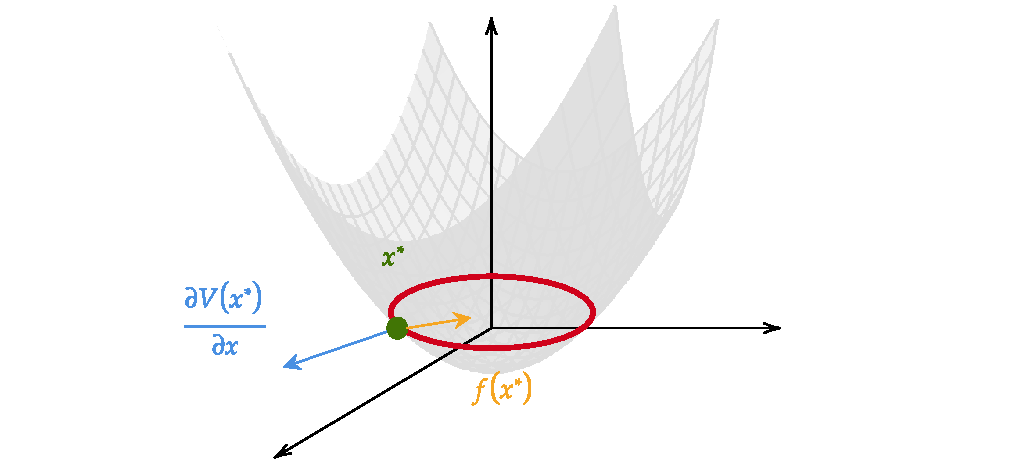
\includegraphics[width=0.75\textwidth]{img/flc_lyap_geom_interp.pdf}
	\caption{Interpretación geométrica de la función de Lyapunov de control.}
	\label{fig: lyapunov_interpretation}
\end{figure}


\rmk{
	Recuerde que aunque la interpretación geométrica es simple, no es fácil encontrar una \gls{flc}.\\
}

Un hecho sorprendente que se concluye de \ref{eq: condicion_flc} es que esto es una \textbf{condición necesaria y suficiente} para que $V(x)$ pueda ser una \gls{flc} para el sistema original, es decir, para que pueda existir una ley de control $\psi(x)$ que estabilice al origen. Si esta condición no se cumple, no puede existir tal ley de control, y esta condición se puede verificar sin necesidad de conocer a $\psi(x)$. De hecho, la existencia de una \gls{flc} es una caracterización de la estabilizabilidad para sistemas no lineales.\\
\rmkb{Entonces, cualquier \gls{fl} para el sistema en lazo cerrado con alguna ley de control que estabilice al origen es una \gls{flc} para el sistema original.}

\rmk{
	La caracterización es entonces extremadamente simple, pues uno no necesita conocer la ley de control para saber que \textbf{existe} una ley de control que estabiliza.
}

\defn{Función de Lyapunov de Control}{
	Una función $V(x)$, continuamente diferenciable y positiva definida, es una \gls{flc} para el sistema
	\begin{equation*}
		\dot{x} = f(x) + g(x)u
	\end{equation*}
	si
	\begin{itemize}
		\item \begin{equation}
			      \dfrac{\partial V(x)}{\partial x} g(x) = 0, \quad \text{para algún} \quad x \in D, x \neq 0 \Rightarrow \dfrac{\partial V(x)}{\partial x} f(x) < 0
			      \label{eq: condicion_flc2}
		      \end{equation}
		\item Satisface la \gls{pcp}.
	\end{itemize}
	Además, es una \gls{flc} global si es \gls{rna} y \eqref{eq: condicion_flc2} se satisface para $D = \mathbb{R}^n$.
}

\thmr{Teorema de Arstein}{arstein_thm}{
	Sea el sistema
	\begin{equation*}
		\dot{x} = f(x) + g(x)u,
	\end{equation*}
	con $f(0) = 0$. Entonces, el origen $x=0$ es \textbf{Globalmente Estabilizable Asintóticamente} por una ley de control de retroalimentación $u = \psi(x)$, continua en todas partes, excepto \textit{posiblemente} en el origen, si y solo si este posee una \gls{flc}. Si además se satisface la \gls{pcp}, entonces la ley de control puede ser continua en todas partes.
}

\section{Fórmula de Sontag}
\thmr{Fórmula de Sontag}{sontag_formula}{
	Sea $V(x)$ una \gls{flc} para el sistema
	\begin{equation*}
		\dot{x} = f(x) + g(x)u
	\end{equation*}
	entonces el origen es estabilizable por
	\begin{equation}
		u = \psi(x) = \begin{cases}
			\dfrac{-\frac{\partial V}{\partial x} f + \sqrt{\left(\frac{\partial V}{\partial x}f\right)^2 + \left(\frac{\partial V}{\partial x}g \right)^4}}{\left(\frac{\partial V}{\partial x}g\right)}, & \text{si } \frac{\partial V}{\partial x}g \neq 0 \\
			0,                                                                                                                                                                                             & \text{si } \frac{\partial V}{\partial x}g = 0.
		\end{cases}
		\label{eq: sontag_formula}
	\end{equation}

	Para el caso multivariable ($u \in \mathbb{R}^m$), se tiene que
	\begin{equation}
		u = \psi(x) = \begin{cases}
			\dfrac{L_f V(x) + \sqrt{[L_f V(x)]^2 + | L_g V(x) |^4}}{| L_g V(x) |^2}[L_g V(x)]^T, & \text{si } | L_g V(x) | \neq 0 \\
			0,                                                                                   & \text{si } | L_g V(x) | = 0.
		\end{cases}
		\label{eq: sontag_formula_multivariable}
	\end{equation}
}

\subsection{Una modificación de la fórmula de Sontag}
Elíjase una función $\gamma(x)$ tal que
\begin{itemize}
	\item $\gamma(x) \geq 0$ y $\gamma(0) = 0$.
	\item Si una solución acotada de la ecuación $\dot{x} = f(x)$ es tal que $\gamma(x(t)) \equiv 0$, entonces $x(t) \rightarrow 0$ cuando $t \rightarrow \infty$, por ejemplo, esto es cierto si $\gamma(x) > 0$ para $x \neq 0$ (detectable de estado cero).
\end{itemize}
\thmr{Fórmula de Sontag Modificada}{sontag_formula_mod}{
	Dada una \gls{flc} $V(x)$, considere la ley de control dada por
	\begin{equation}
		u = \psi(x) = \begin{cases}
			\dfrac{L_f V(x) + \sqrt{[L_f V(x)]^2 + \textcolor{red}{\gamma(x)}| L_g V(x) |\textcolor{red}{^2}}}{| L_g V(x) |^2}[L_g V(x)]^T, & \text{si } | L_g V(x) | \neq 0 \\
			0,                                                                                                                              & \text{si } | L_g V(x) | = 0.
		\end{cases}
		\label{eq: sontag_formula_mod}
	\end{equation}
}

\rmk{Nótese que:}
\begin{itemize}
	\item La elección de $\gamma(x) = |L_g V(x)|^2$ satisface los requisitos anteriores y se recupera la fórmula de Sontag.
	\item Hay muchas otras elecciones posibles de $\gamma(x)$: \textbf{Gran flexibilidad}.
\end{itemize}
\rmk{¿Cuáles son las propiedades de esta ley de control modificada?}
\begin{itemize}
	\item $\psi(x)$ hace que el \gls{pe} $x=0$ sea \gls{gae}.
	\item $\psi(x)$ es tan suave como $L_f V$, $L_g V$ y $\gamma(x)$, excepto (posiblemente) donde $\gamma(x) = L_f V (x) = 0$.
	\item Si $L_f V, L_g V$ y $\gamma(x)$ son localmente Lipschitz, entonces $\psi(x)$ también lo será, excepto (posiblemente) en el origen $x=0$.
	\item Si $V(x)$ tiene los mismos conjuntos de nivel que la solución de la ecuación de Hamilton-Jacobi-Bellman, asociada con la función de costo
	      \begin{equation*}
		      J = \int_0^\infty [\gamma(x(\tau)) + |u(\tau)|^2] d\tau
	      \end{equation*}
	      entonces $\psi(x)$ es óptima globalmente.
	\item Este hecho se puede usar para diseñar leyes de control localmente óptimas.
\end{itemize}

\rmkb{
	\textbf{Problema: ¿Cómo se puede encontrar una \gls{flc}?}

	Las propiedades de \gls{flc} y \gls{pcp} se preservan ante transformaciones de retroalimentación, es decir, retroalimentación y cambio de coordenadas (difeomórficas).\\

	Si se conoce algún control estabilizante y una \gls{fl} correspondiente $V$, entonces $V$ es una \gls{flc}.\\

	Principalmente, se verán dos formas de encontrar una \gls{flc}:
	\begin{itemize}
		\item Feedback Linearization
		\item Backstepping
	\end{itemize}
}



\subsection{FLC por Feedback Linearization}
Por este método es relativamente simple encontrar una \gls{flc}, ya que es muy simple estabilizar el sistema y encontrar una \gls{fl} para el sistema en lazo cerrado.\\

Considere el sistema
\begin{equation*}
	\dot{x} = f(x) + G(x)u, \quad z = T(x), \quad \dot{z} = (A-BK)z
\end{equation*}
Resolviendo la ecuación algrebraica de Lyapunov
\begin{equation*}
	(A-BK)^T P + P(A-BK) = -Q, \quad Q = Q^T > 0
\end{equation*}
Entonces
\begin{equation*}
	V(x) = z^T P z = T(x)^T P T(x)
\end{equation*}
es una \gls{flc} para el sistema original.\\

\rmkb{
	Una ley de control estabilizante alternativa para sistemas linealizables exactamente se puede obtener de la siguiente manera:
	\begin{itemize}
		\item Encuentre una \gls{flc} para el sistema \gls{lit} transformado (resolviendo la ecuación algebraica de Lyapunov).
		\item Use la fórmula de Sontag en vez de la ley de control linealizante.
	\end{itemize}
}

\ex{
	\begin{equation*}
		\dot{x} = ax - bx^3 + u, \quad a, b > 0
	\end{equation*}
	Linealización por retroalimentación:
	\begin{equation*}
		u = -(k+a)x + bx^3, \quad k > 0, \quad \Rightarrow \quad \dot{x} = -kx
	\end{equation*}
	Entonces, $V(x) = \dfrac{1}{2}x^2$ es una \gls{flc}.\\
	Luego,
	\begin{equation*}
		\dfrac{\partial V(x)}{\partial x} g(x) = x, \quad \dfrac{\partial V(x)}{\partial x} f(x) = x(ax - bx^3)
	\end{equation*}
	Usando la fórmula de Sontag:
	\begin{equation*}
		\begin{aligned}
			\psi(x) & = -\dfrac{x(ax - bx^3) + \sqrt{x^2(ax - bx^3)^2 + x^4}}{x} \\
			        & = -ax + bx^3 - x\sqrt{(a-bx^2)^2 + 1}
		\end{aligned}
	\end{equation*}
	Compare lo anterior con
	\begin{equation*}
		u = -ax + bx^3 -kx, \quad k > 0
	\end{equation*}
}

\lem{}{
	Sea $V(x)$ una \gls{flc} para el sistema
	\begin{equation*}
		\dot{x} = f(x) + g(x)u
	\end{equation*}
	y supóngase que
	\begin{equation*}
		\dfrac{\partial V(0)}{\partial x} = 0,
	\end{equation*}
	entonces la fórmula de Sontag tiene un margen de ganancia de $[\frac{1}{2},\infty]$, es decir, $u = k\psi(x)$ es estabilizante para toda $k \geq \frac{1}{2}$.
}










%%%%%%%%%%%%%%%%%%%%%%%%%%%%%%%%%%%%%%%%%%%%%%%%%%%%%%%%%%%%%%%%%%%%%%%%%%%%%%%%%%%%%%%%%%%%%%%%%%%%%%%
% Capítulo 7: Backstepping
%%%%%%%%%%%%%%%%%%%%%%%%%%%%%%%%%%%%%%%%%%%%%%%%%%%%%%%%%%%%%%%%%%%%%%%%%%%%%%%%%%%%%%%%%%%%%%%%%%%%%%%

\chapter{Backstepping}
Este es un método para construir una \gls{flc} para una clase especial de sistemas.\\

\rmk{
	También se puede encontrar en la literatura el \textit{Forwarding}, pero no se aborda debido a que es, en general, un método más complicado.
}
\section{El caso más simple: Backstepping de integrador}
La idea básica del método conocido como \textbf{backstepping} es la siguiente se puede expñlicar, en su forma más simple, considerando el sistema con entrada escalar
\begin{equation}
	\begin{aligned}
		\dot{\eta} & = f(\eta) + g(\eta)\xi                                    \\
		\dot{\xi}  & = u, \quad \eta \in \mathbb{R}, \quad \xi \in \mathbb{R}.
	\end{aligned}
	\label{eq: backstepping_integrador}
\end{equation}
Nótese que este sistema se puede ver como una conexión en cascada, donde el maestro es un integrador y el esclavo es el sistema no lineal $\dot{\eta} = f(\eta) + g(\eta)\xi$. El objetivo de control es estabilizar el origen utilizando retroalimentación de los estados.\\

La idea de Backstepping es escencialmente recursiva, es decir, partimos de pensar en $\xi$ como una variable de control \textit{virtual} para el sistema $\dot{\eta} = f(\eta) + g(\eta)\xi$ y queremos diseñar una ley de control para $\xi$ que estabilice al origen asintóticamente, es decir, buscamos estabilizar al esclavo de la cascada. La idea básica descrita a bloques se puede apreciar en la Figura \ref{fig: backstepping_bloques}.\\

\begin{figure}[H]
	\centering
	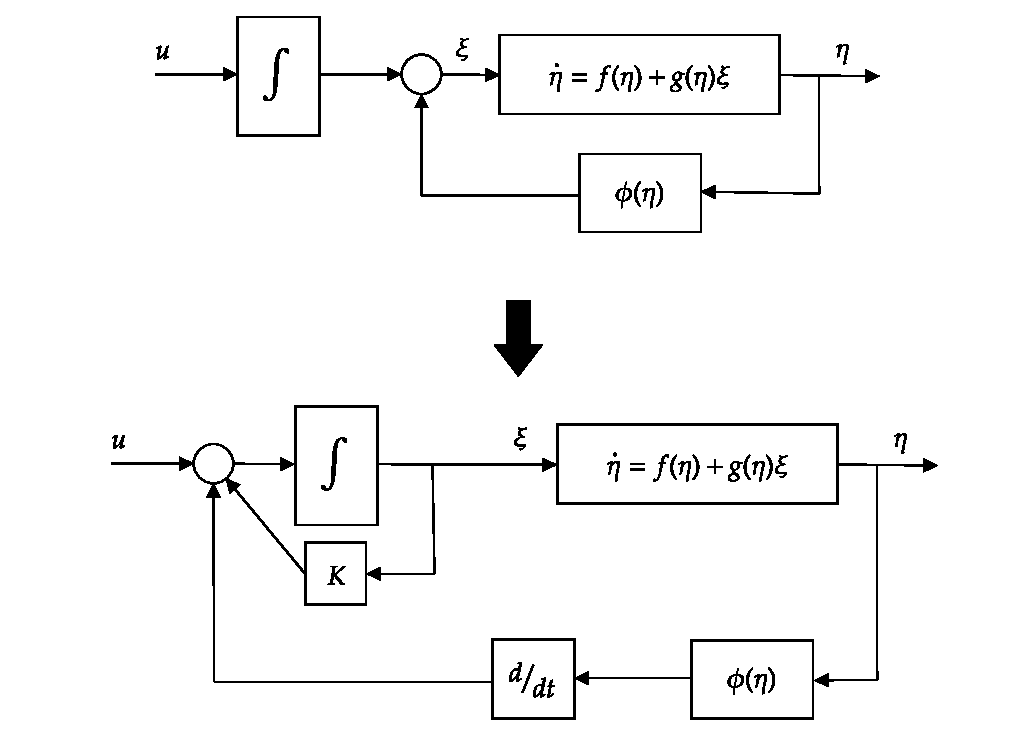
\includegraphics[width=0.8\textwidth]{img/backstepping_BlockDiagram.pdf}
	\caption{Idea básica del Backstepping de integrador.}
	\label{fig: backstepping_bloques}
\end{figure}

\subsection{Diseño del control virtual}
Véase a $\xi$ como una entrada de control virtual del sistema
\begin{equation}
	\dot{\eta} = f(\eta) + g(\eta)\xi.
	\label{eq: backstepping_esclavo}
\end{equation}
Suponga que existe una ley de control retroalimentado
\begin{equation*}
	\xi = \phi(\eta)
\end{equation*}
que estabiliza el origen de
\begin{equation*}
	\dot{\eta} = f(\eta) + g(\eta)\phi(\eta).
\end{equation*}
y que, además, conocemos una \gls{fl} $V(\eta)$ que lo asegura:

\begin{equation*}
	\dot{V}(\eta) = \dfrac{\partial(\eta)}{\partial \eta} [f(\eta) + g(\eta)\phi(\eta)] \leq -W(\eta), \quad \forall \eta \in D.
\end{equation*}

\subsection{Diseño del control verdadero por Backstepping}
\textbf{Cambio de coordenadas:} Como no se puede implementar el control virtual $\xi = \phi(\eta)$, definimos el error como una nueva variable
\begin{equation*}
	z = \xi - \phi(\eta).
\end{equation*}
Escribiendo el sistema en términos de esta nueva variable se obtiene
\begin{equation*}
	\begin{aligned}
		\dot{\eta} & = [f(\eta) + g(\eta)\phi(\eta)] + g(\eta)z,                                                         \\
		\dot{z}    & = u - \frac{\partial \phi(\eta)}{\partial \eta} [f(\eta) + g(\eta)\xi], \quad \xi = z + \phi(\eta).
	\end{aligned}
\end{equation*}
Si se diseña la variable de control como
\begin{equation*}
	u = -\dfrac{\partial \phi(\eta)}{\partial \eta} [f(\eta) + g(\eta)\xi] + v
\end{equation*}
entonces el sistema se describe como
\begin{equation}
	\begin{aligned}
		\dot{\eta} & = [f(\eta) + g(\eta)\phi(\eta)] + g(\eta)z, \\
		\dot{z}    & = v.
	\end{aligned}
	\label{eq: backstepping_z}
\end{equation}
\rmkb{
	¿Cuál es la diferencia entre \eqref{eq: backstepping_esclavo} y \eqref{eq: backstepping_z}? La diferencia es que en \eqref{eq: backstepping_z} el esclavo con la entrada proveniente del maestro igualada a cero $(z=0)$ tiene un \gls{pe} que es asintóticamente estable, esto es, el sistema es de Fase Mínima.\\

	En resumen, con un simple cambio de variables estabilizamos la \gls{dc} del sistema.\\

	Bastaría con estabilizar al maestro (que ya es lineal) y entonces el sistema completo tiene un \gls{pe} asintóticamente estable localmente (usando las ideas de linealización parcial).
}
La diferencia ahora, sin tomar el camino de Linealización Parcial, será construir una \gls{flc} para el sistema \eqref{eq: backstepping_z}, luego vamos a usar esa \gls{flc} para estabilizar al sistema completo \eqref{eq: backstepping_integrador}.

\subsubsection{Diseño del control por Lyapunov} El diseño se realiza proponiendo una \textbf{función candidata de Lyapunov}, en nuestro caso se puede usar
\begin{equation*}
	V_c(\eta, \xi) = V(\eta) + \dfrac{1}{2}z^2.
\end{equation*}
El control $v$ se elige de tal forma que $\dot{V}_c$:
\begin{equation*}
	\dot{V}_c = \underbrace{\dfrac{\partial V}{\partial \eta} [f(\eta) + g(\eta)\phi(\eta)]}_{<0} + \underbrace{\dfrac{\partial V(\eta)}{\partial \eta}g(\eta)z + zv}_{\text{diseñe } v}.
\end{equation*}
sea negativa definida. Aquí se propone
\begin{equation*}
	v = -\dfrac{\partial V(\eta)}{\partial \eta}g(\eta)z - kz, \quad k > 0.
\end{equation*}
con lo que
\begin{equation*}
	\dot{V}_c \leq -W(\eta) -kz^2,
\end{equation*}
donde
\begin{equation*}
	W(\eta) = \dfrac{\partial V(\eta)}{\partial \eta}g(\eta)z^2 - \dfrac{\partial V(\eta)}{\partial \eta}g(\eta)z.
\end{equation*}
El control $u$ finalmente, resulta ser
\begin{equation*}
	u = -\dfrac{\partial \phi(\eta)}{\partial \eta} [f(\eta) + g(\eta)\xi] - \dfrac{\partial V(\eta)}{\partial \eta}g(\eta)z - k(z + \phi(\eta)), \quad k > 0.
\end{equation*}
\rmkb{
	Note las siguientes diferencias importantes con respecto a la Linealización Parcial:
	\begin{itemize}
		\item La suma de las funciones de Lyapunov para los sistemas individuales se convierte en una función de Lyapunov para el sistema completo. Esto es gracias a la acción de control.

		\item El subsistema esclavo de la cascada no tiene que ser estable con entrada cero, sino que se puede estabilizar mediante el control virtual.
	\end{itemize}
}





%%%%%%%%%%%%%%%%%%%%%%%%%%%%%%%%%%%%%%%%%%%%%%%%%%%%%%%%%%%%%%%%%%%%%%%%%%%%%%%%%%%%%%%%%%%%%%%%%%%%%%%
% Capítulo 8: Pasividad
%%%%%%%%%%%%%%%%%%%%%%%%%%%%%%%%%%%%%%%%%%%%%%%%%%%%%%%%%%%%%%%%%%%%%%%%%%%%%%%%%%%%%%%%%%%%%%%%%%%%%%%

\chapter{Control basado en Pasividad}
\label{chap:control-pasividad}

La \textbf{pasividad} es una propiedad fundamental que poseen ciertos sistemas dinámicos y puede ser aprovechada para el diseño de controladores. Se trata de un enfoque que, a diferencia del método clásico de Lyapunov, se basa explícitamente en el análisis de la relación entre \textit{entradas y salidas}, ya sean físicas o introducidas de manera ficticia.\\

En términos generales, un sistema se considera pasivo si cumple con un \textit{principio de conservación de energía}: la energía que entra al sistema no puede ser menor que la energía que se almacena en él. Para analizar esta propiedad, se asocia al sistema una función escalar \( V(x) \), conocida como \textit{función de almacenamiento}, que representa la energía almacenada. Esta función debe ser al menos continua, diferenciable y al menos semidefinida positiva.\\

La pasividad se evalúa a través de un balance energético. La \textit{potencia suministrada} al sistema se modela como el producto interno entre la entrada \( u(t) \) y la salida \( y(t) \), es decir, \( u^T y \). Si el sistema es pasivo, entonces la derivada temporal de la energía almacenada debe ser menor o igual a la potencia suministrada:

\begin{equation*}
	\dot{V}(x) \leq u^T y.
\end{equation*}

Esto implica que el sistema no genera energía internamente: toda la energía almacenada proviene del exterior. Si por el contrario \( \dot{V}(x) > u^T y \), entonces el sistema tendría fuentes internas de energía y no sería pasivo.\\

Otra forma intuitiva de verlo, es que si uno NO aplica ninguna entrada a un sistema pasivo, la energía de este sistema no puede crecer, entonces lo más que le puede ocurrir a la energía de este sistema es que se quede estática o que disminuya. Una implicación inmediata, entonces, es que, si la función de energía cumple las condiciones que pide el teorema de Lyapunov (es positiva definida), entonces el origen es un \gls{pe} estable (no necesariamente asintóticamente estable).

\section{Idea básica}
Considere el sistema
\begin{equation}
	\Sigma : \left\{
	\begin{aligned}
		 & \dot{x} = f(x,u), \quad x \in \mathbb{R}^n, u \in \mathbb{R}^p \\
		 & y = h(x), \quad \quad y \in \mathbb{R}^m
	\end{aligned}
	\right.
	\label{eq:sistema_pasivo}
\end{equation}
\begin{equation*}
	f(0,0) = 0, \quad h(0) = 0
\end{equation*}

\defn{Sistema Pasivo}{
	El sistema es \textbf{pasivo} si existe una función de almacenamiento de energía \( V(x) \), continuamente diferenciable y positiva semidefinida, tal que
	\begin{equation}
		\dot{V}(x) = \frac{\partial V}{\partial x} f(x,u) \leq u^T y, \quad \forall x \in \mathbb{R}^n, u \in \mathbb{R}^p
	\end{equation}
}
La siguiente definición, conocida como \textit{observabilidad de estado cero}, nos habla de cuándo podemos determinar que el sistema está en estado cero a partir de la entrada y la salida, esto no necesariamente significa que podamos determinar el estado del sistema, sino que podemos determinar si el sistema está en equilibrio o no.\\
\defn{Observabilidad de estado cero}{
	El sistema es de \textbf{observable de estado cero} si la única trayectoria del sistema con entrada $u = 0$
	\begin{equation*}
		\dot{x} = f(x,0)
	\end{equation*}
	que puede hacer la salida cero, es decir, que puede permanecer en el conjunto ${h(x) = 0}$ es la solución trivial $x(t) \equiv 0$.\\
}
Un resultado básico de estabiliziación asintótica para sistemas pasivos se enuncia en el siguiente teorema.
\thmr{}{}{
	Si el sistema \eqref{eq:sistema_pasivo} es
	\begin{itemize}
		\item pasivo, con función de almacenamiento positiva definida y radialmente no acotada, y
		\item de estado cero observable
	\end{itemize}
	entonces el origen es $x=0$ puede ser estabilizado global y asintóticamente mediante la ley de control
	\begin{equation*}
		u = -\phi(y)
	\end{equation*}
	donde $\phi(y)$ es cualquier función localmente Lipschitz, tal que $\phi(0) = 0$ y es pasiva
	\begin{equation*}
		y^T \phi(y) \geq 0, \quad \forall y \neq 0
	\end{equation*}
}
\pf{
	Use la función de almacenamiento $V(x)$ como candidata a \gls{fl} para el sistema en lazo cerrado
	\begin{equation*}
		\dot{x} = f(x, -\phi(y)).
	\end{equation*}
	Su derivada es
	\begin{equation*}
		\dot{V}(x) = \frac{\partial V}{\partial x} f(x, u) \leq -y^T \phi(y) \leq 0
	\end{equation*}
	negativa semidefinida. Además $\dot{V}(x) = 0$ sólo si $y = 0$. De la propiedad de estado cero observable se concluye
	\begin{equation*}
		y(t) \equiv 0 \implies u(t) = -\phi(y(t)) \equiv 0 \implies x(t) \equiv 0
	\end{equation*}
	y por el principio de invarianza de LaSalle, el origen es global y asintóticamente estable.
}

\rmkb{
	\begin{itemize}
		\item Recuerde que, si la función de almacenamiento es positiva definida, el origen del sistema pasivo es estable, y que la interconexión en retroalimentación negativa de sistemas pasivos es pasiva. Por lo tanto, el teorema se puede interpretar de la siguiente manera: \textbf{la no linealidad pasiva $\phi$ inyecta amortiguamiento al sistema, haciendo que las trayectorias converjan al origen.}
		\item Note que hay una gran libertad de elección en la forma de la función de inyección de amortiguamiento $\phi$: por ejemplo, se pueden satisfacer restricciones de acotamiento de la entrada.
		\item Ya que el teorema sólo es útil para sistemas pasivos, su utilidad se incrementa si se pueden convertir sistemas no pasivos en pasivos \textbf{(Pasivización)}.
	\end{itemize}
}

Hay dos formas básicas de hacer pasivo a un sistema:
\begin{enumerate}
	\item Mediante la selección de la salida,
	\item por retroalimentación de estados, o ambas.
\end{enumerate}

\section{Pasivización por selección de salida}
Considere el sistema afín en las entradas
\begin{equation}
	\dot{x} = f(x) + G(x)u
	\label{eq:sistema_af}
\end{equation}
y suponga que existe una función $V(x)$ continuamente diferenciable, positiva definida, tal que

\begin{equation*}
	\dot{V}(x) = \frac{\partial V}{\partial x} f(x) \leq 0, \quad \forall x
\end{equation*}

Entonces, el sistema es pasivo con respecto a la salida
\begin{equation*}
	y = h(x) \overset{\Delta}{=} \left[ \dfrac{\partial V(x)}{\partial x} G(x) \right]^T,
\end{equation*}
ya que
\begin{equation*}
	\dot{V}(x) = \frac{\partial V}{\partial x} [ f(x) + G(x)u] \leq \frac{\partial V}{\partial x} G(x)u = y^T u .
\end{equation*}
Si adicionalmente es de estado cero observable, entonces puede utilizarse el teorema para estabilizar asintóticamente el origen.

\rmkb{
	Nótese que no existe una única salida pasiva. Para cada elección de $V(x)$, se obtiene (posiblemente) una salida pasiva difirente.
	Considere, por ejemplo, como \gls{fl} alternativa
	\begin{equation*}
		W(x) = \gamma(V(x))
	\end{equation*}
	donde $\gamma$ una función tipo $\mathcal{K}$, continuamente diferenciable ($\mathcal{K}_\infty$ para el caso global). Entonces una salida pasiva con esta \gls{fl} sería

	\begin{equation*}
		\tilde{y} = \tilde{h}(x) \overset{\Delta}{=} \left[ \dfrac{\partial W(x)}{\partial x} G(x) \right]^T = \gamma'(V(x)) \left[ \dfrac{\partial V(x)}{\partial x} G(x) \right]^T = \gamma'(V(x)) h(x)
	\end{equation*}
}
\ex{
	\begin{equation*}
		\begin{aligned}
			 & \dot{x}_1 = x_2        \\
			 & \dot{x}_2 = -x_1^3 + u
		\end{aligned}
	\end{equation*}
	con $u = 0$
	\begin{equation*}
		V(x) = \dfrac{1}{4} x_1^4 + \dfrac{1}{2} x_2^2 \implies \dot{V}(x) = x_1^3 x_2 - x_2 x_1^3 = 0
	\end{equation*}
	El sistema es pasivo con respecto a la salida
	\begin{equation*}
		y = \dfrac{\partial V(x)}{\partial x} G(x) = \dfrac{\partial V(x)}{\partial x_2} = x_2
	\end{equation*}
	Es decir, la salida pasiva es la velocidad del sistema.\\
	\rmk{¿Es de estado cero observable? Si.\\}
	con
	\begin{equation*}
		u = 0, y(t) \equiv 0 \implies x(t) \equiv 0
	\end{equation*}
	Aplicando el teorema, el origen e puede estabilizar global y asintóticamente con cualquier $\phi$ pasiva, por ejemplo
	\begin{equation*}
		u = -k x_2, \quad \text{o} \quad u = \left( \dfrac{2k}{\pi} \right) \tan^{-1} x_2, k > 0
	\end{equation*}
}

\section{Pasivización por retroalimentación de estados}
La pasivización por elección de la salida exige que el sistema tenga un punto de equilibrio estable, por lo que muchos sistemas no pueden ser pasivizados por tal método. Para poder considerar sistemas no estables, se requiere utilizar una retroalimentación preliminar.\\

\defn{}{
	El sistema
	\begin{equation*}
		\Sigma_A : \left\{
		\begin{aligned}
			 & \dot{x} = f(x) + G(x)u, \quad x \in \mathbb{R}^n, u \in \mathbb{R}^p \\
			 & y = h(x), \quad \quad y \in \mathbb{R}^p
		\end{aligned}
		\right.
	\end{equation*}
    es equivalente por retroalimentación a un sistema pasivo si existe
    \begin{equation*}
        u = \alpha(x) + \beta(x) v
    \end{equation*}
    tal que
    \begin{equation*}
        \begin{aligned}
            \dot{x} &= f(x) + G(x)\alpha(x) + G(x) \beta(x) v, \quad x \in \mathbb{R}^n, v \in \mathbb{R}^p\\
            y &= h(x), \quad \quad y \in \mathbb{R}^p
        \end{aligned}
    \end{equation*}
    sea pasivo.
}
\rmkb{
    Esta definición es análoga a la de sistemas linealizables por retroalimentación. Una diferencia importante es que en la de pasivización no se requiere de una transformación de estados, ya que la pasividad, a diferencia de la linealidad, es una propiedad invariante ante transformaciones del estado.\\
}




%%%%%%%%%%%%%%%%%%%%%%%%%%%%%%%%%%%%%%%%%%%%%%%%%%%%%%%%%%%%%%%%%%%%%%%%%%%%%%%%%%%%%%%%%%%%%%%%%%%%%%%
\defn{Relative Degree}{

}


\defn{Definition Name}{
	A defintion.
}

\thmr{Theorem Name}{mybigthm}{
	A theorem.
}

\lem{Lemma Name}{
	A lemma.
}

\fact{
	A fact.
}

\cor{
	A corollary.
}

\prop{
	A proposition.
}

\clmp{}{
	A claim.
}{
	A reference to Theorem~\ref{thm:mybigthm}
}

\pf{
	Veniam velit incididunt deserunt est proident consectetur non velit ipsum voluptate nulla quis. Ea ullamco consequat non ad amet cupidatat cupidatat aliquip tempor sint ea nisi elit dolore dolore.

	Laboris labore magna dolore eiusmod ea ex et eiusmod laboris. Et aliquip cupidatat reprehenderit id officia pariatur.
}

\ex{
	Nostrud esse occaecat Lorem dolore laborum exercitation adipisicing eu sint sunt et. Excepteur voluptate consectetur qui ex amet esse sunt ut nostrud qui proident non. Ipsum nostrud ut elit dolor. Incididunt voluptate esse et est labore cillum proident duis.
}

\rmk{
	Some remark.
}

\rmkb{
	Some more remark.
}

\section{Pictures}

% \begin{figure}[H]
%     \center
%     \includegraphics[scale=0.1]{img/loo.jpg}
%     \caption{Waterloo, ON}
% \end{figure}

\printbibliography[title=Referencias]
\end{document}
